\chapter[FAST observations of an MSP]{Curious single-pulse modulation in the millisecond pulsar J1518+4904}
\label{chapt: J1518}

This chapter details observations of PSR~J1518+4904, a millisecond pulsar in a binary system which, along with PSRs J1012+5307 and J1713+0747, is one of three MSPs with known drifting subpulses. The observations were performed with FAST during its commissioning phase. These observations are part of a programme to exploit the sensitivity of the telescope to produce `technical test and science demonstration data' to allow the study of timing noise in pulsars. The observations revealed two previously unknown profile components that greatly extend the overall pulse width, and multiple distinct periodicities in the single pulse data which seem to happen simultaneously. It therefore cannot be attributed to mode-switching behaviour. In addition to the distinct periodicities, there also appears to be a smooth pulse longitude dependence of the fluctuation frequency across different pulse profile components, which cannot be explained with existing models of the production of radio emission in pulsars.

\section{Introduction}
\label{sec: J1518 - intro}

PSR~J1518+4904 is a millisecond binary pulsar with a period of 40.9~ms discovered in the Green Bank Northern Sky Survey \citep{NSTx1996,SNTx1997}. Its companion is a neutron star, making it one of at least 15 known double neutron star (DNS) systems \citep{TKF+2017}. PSR~J1518+4904 has a mean flux density of $2.5\pm2$~mJy at 1.4~GHz \citep{LKG+2016} and is a recycled pulsar. Recycled pulsars are older objects which accrete matter from their binary companions, transferring angular momentum to the pulsar and causing it to spin-up to a typical rotational speed of hundreds of rotations per second \citep[e.g.][]{PulsarAstronomy}. An overview of the pulsar population is given in Sec.~\ref{sec: intro - general intro - pulsar population}.% Recycled pulsars are objects which have at some point in the past undergone mass accretion from their binary companion; this causes them to spin-up to a typical rotational speed of hundreds of rotations per second \citep[e.g.][]{PulsarAstronomy}. Before spin-up these were older, normal pulsars, decaying in luminosity as they lose energy -- the increase in rotational energy through accretion rejuvenates them causing them to once again emit radio waves. An overview of the pulsar population is given in Sec.~\ref{sec: intro - general intro - pulsar population}.

Previous studies have found that PSR~J1518+4904 has a relatively narrow pulse profile compared to many other millisecond pulsars (MSPs), with a duty cycle $W_{10} = 5.4\pm0.2$~per~cent compared to an mean of $\langle W_{10} \rangle= 21$~per~cent across the MSP population  at 1.4~GHz \citep{KXL+1998}. The integrated profiles of MSPs are generally much wider than those of ordinary pulsars, and are often more complex with more components \citep[e.g.][]{YMS+2011}, although their spectral properties are similar \citep{TBMS1998, KXL+1998, KLL+1999}. By investigating and comparing the radio properties and $\gamma$-ray beaming of MSPs and normal pulsars, \citet{Mxxx2005} and \citet{RMHx2010} suggest that the radio emission of MSPs is produced at high altitudes within the magnetosphere (as a fraction of the light cylinder radius) -- possibly the `outer gap' which is usually associated with high-energy emission \citep[e.g.][]{CZxx1998} -- resulting in very wide beams. \citet{NSTx1996} studied PSR~J1518+4904 between 320 and 1400~MHz, and their data show a double-peaked profile with a stronger leading component, and a broad tail at the lower frequencies. This pulsar was part of a study of the properties of MSPs by \citet{KXL+1998} who discovered that the profile shows a postcursor at 1.4~GHz. The postcursor is separated from the centre of the main profile by approximately $25\degr$, but is connected to it by low-intensity emission. A subsequent multi-frequency study of the pulsar \citep{KLL+1999} showed that this postcursor disappears at higher frequencies, and also at lower frequencies because it becomes swamped by the tail of the main component \citep{NSTx1996,STCx1999}.


PSR~J1518+4904 was initially selected for observation by the Five-hundred-metre Aperture Spherical radio Telescope (FAST) during commissioning to test the telescope performance and capabilities, but also because it is a promising source to study `jitter noise'. Jitter noise is related to the fact that the individual pulses of pulsars are variable in shape (for example due to effects described in Sec.~\ref{sec: intro - emission models - single pulse phenomena}). This affects the precision with which arrival times can be measured, hence resulting in uncertainties in the timing precision of pulsars. This stochastic uncertainty comes on top of potentially correlated `red' timing noise which represents unmodeled variations in the spin-down of pulsars. The rapid rotation of MSPs means that typically large numbers of pulses are collected in a single observation, thereby averaging out much (but not all) of the jitter noise. The high precision in timing for a small selection of the MSP population makes them ideal probes to try to detect gravitational waves \citep[e.g.][]{FBxx1990,MHB+2013}, which affect pulse arrival times by very small amounts. A better understanding of timing noise can be crucial in order to achieve the highest possible timing precision, thus maximising the sensitivity for detecting gravitational waves. A large telescope such as FAST can provide the most sensitive arrival time measurements, and is ideal to study the pulse-to-pulse variations in the pulse shape of MSPs as their individual pulses can be detected with enough significance.


Quasi-periodic modulation was detected throughout the main profile component of PSR~J1518+4904 by \citet{ESxx2003} using 1650 single pulses from archival data at 1.4~GHz recorded using the Westerbork Synthesis Radio Telescope (WSRT). Using a two-dimensional fluctuation spectrum (2DFS, as described in Sec.~\ref{sec: J1926 - analysis - single pulse variability}), they detected modulation with frequency $P_3\sim0.38$~cpp and $P_2\sim 10$~cpp (see Sec.~\ref{sec: intro - emission models - single pulse phenomena} for the definition of $P_2$ and $P_3$). 
A motivation for developing the 2DFS by \citet{ESxx2002} was to be able to detect periodic pulse shape variations even when the pulsar signal is not strong enough to detect the individual pulses with high significance, making the results of \citet{ESxx2003} especially satisfying. The positive value of $P_2$ demonstrates that PSR~J1518+4904 has drifting subpulses that move rapidly from earlier longitudes to later longitudes across the pulse profile\footnote{In the original paper $P_2$ was quoted as negative -- this is due to a different convention in the sign. In this thesis, a positive $P_2$ corresponds to drift towards later longitudes.}. This finding, along with similar behaviour in PSR~J1012+5307, was the first ever detection of drifting subpulses in recycled pulsars \citep{ESxx2003}, suggesting that the magnetospheric physics might be very similar in MSPs and slower pulsars, despite their vastly different light-cylinder radii (see Sec.~\ref{sec: intro - general intro - pulsar population}). This knowledge led us to propose additional observations of PSR~J1518+4904 to be performed with FAST after the existing observation aimed at studying the jitter noise, in order to study this modulation behaviour in unprecedented detail.

Drifting subpulses were later discovered in another MSP, PSR~J1713+0747 \citep{LBJ+2016}. This finding increases the known number of MSP drifters to three -- however, given that high-sensitivity searches for drifting subpulses have been performed for only approximately ten MSPs, the phenomenon does not appear to be unusual, and is comparable to what is found for the non-recycled pulsar population \citep[more than 55~per~cent;][]{WESx2007}. All three MSPs are classified as `diffuse' drifters by the definition of \citet{WESx2006}. These are pulsars which have a vertically broad $P_3$ feature in their spectra, in contrast with `coherent' drifters which have well-defined, narrow $P_3$ features that indicate that the periodicity of the pulse-to-pulse modulation is stable throughout the observation. In a sample of 192 (mostly non-recycled) pulsars \citep[Table 2]{WESx2006} 21 were identified as coherent drifters and 51 as diffuse drifters, meaning that unstable $P_3$ appears to be commonplace. 

This chapter is structured as follows. In Sec.~\ref{sec: J1518 - observations} the observations are summarised, along with the properties of the processed data that were available for analysis. In Sec.~\ref{sec: J1518 - analysis - new profile component} we present the discovery of two new profile components. In Sec.~\ref{sec: J1518 - analysis - LRFS} and Sec.~\ref{sec: J1518 - analysis - 2DFS} we investigate the single-pulse modulation and drifting behaviour, and show that there are at least two distinct periodicities present. In Sec.~\ref{sec: J1518 - analysis - drifting P3} we highlight that in the main part of the profile the periodicity appears to be pulse longitude-dependent. We show in Sec.~\ref{sec: J1518 - analysis - disjoint modes} that there is no evidence that these are the result of distinct switches such that only one periodicity is present at a given time. We also explore the longitude-resolved auto- and cross-correlation functions to highlight this longitude-dependent periodicity further in Sec.~\ref{sec: J1518 - analysis - correlation}. We discuss the implications of the extra profile components and highlight the complications in explaining the observed drifting subpulses with current theory in Sec.~\ref{sec: J1518 - discussion}.


\section{Summary of observations}
\label{sec: J1518 - observations}

PSR~J1518+4904 was initially observed on 13 July 2018 in a trial observation to establish whether its single pulses could be detected by FAST. This observation consisted of 44,000 single pulses, and was unfortunately dominated by radio-frequency interference (RFI). Therefore, a second attempt to observe the pulsar was made on 22 July 2018, and this resulted in a far better detection of the pulsar. This observation consists of 46,000 single pulses at a resolution of 512 pulse longitude bins per period. Two more observations were made on 4 August and 4 November 2018. Both of these were divided into eight frequency sub-bands in post-processing after the observation to investigate the spectral properties of the single pulses. The August observation consists of 43,900 single pulses, whilst the November observation contains 88,400 single pulses and consequently its integrated profile has the highest signal-to-noise ratio (S/N). A summary of the available data is shown in Table~\ref{tab: J1518 - observation summary}.

\begin{table}
    \centering
    \caption[PSR~J1518+4904 available data summary]{A summary of the available data for the four observations that were made of PSR~J1518+4904. The first observation (marked with a *) was strongly affected by RFI, so is not considered further in the analysis. All observations were recorded with a centre frequency of 1250~MHz and a bandwidth of 500~MHz. }
    \label{tab: J1518 - observation summary}
    \begin{tabular}{lccccccc}
        \hline
        Date & Nr. single & Duration & Nr. bins & Freq. & S/N & Pol.\\
         & pulses & (mins) & & channels & & channels\\
        
        \hline
        2018-07-13 * & 44000 & 30 & 512 & 4096 & --& 2\\ 
        2018-07-22 & 46000 & 30 & 512 & 4096 & $2.19\times10^5$ & 2\\
        2018-08-04 & 43900 & 30 & 512 & 4096 & $0.71\times10^5$ & 2\\
        2018-11-04 & 88400 & 60 & 512 & 4096 & $3.00\times10^5$ & 4
    \end{tabular}
\end{table}

The length of the first three observations was 30 minutes, and these were performed in `search mode' (i.e. recorded as a time-series rather than performing on-line folding during the observation), and using the ROACH2 backend and (at the time) newly installed 19-beam receiver \citep[e.g][]{JYG+2019}. The ROACH2 backend processed a bandwidth of 500~MHz centred at 1250~MHz, divided into 4096 frequency channels. The sampling time was 49.152~$\upmu$s. For the final discussed observation, recorded on 2018-11-04, the observation was extended to one hour. 

The number of polarisation channels for the first three observations was two -- this means that only the power (auto-correlations) of the $x$- and $y$-elements of the crossed dipole antennas in the receiver were recorded. These can be combined to effectively give the total power received. For the 2018-11-04 observation four channels were recorded, with the extra channels corresponding to the cross correlation between the two elements (which includes phase information). In theory, this means full polarisation information was captured. A pulsed noise diode signal was observed both before and after this observation which is done with the aim to perform polarisation calibration. However, because of the lack of a receiver solution at the time during commissioning, and because there were slight gain differences unaccounted for between the polarisation channels which remained uncorrected, this meant that accurate calibration was not possible. As a consequence, the polarisation information is unreliable. Given that the profile of PSR~J1518+4904 is known to be largely unpolarised \citep{XKJ+1998, STCx1999,HDSL2009}, even observing this pulsar with only two polarisation channels ought to produce data that resembles Stokes $I$. Nevertheless, this limitation on the described data makes it possible that some apparent variability in the data in fact relates to variability in the polarisation state of the pulsar. The conclusions in this chapter are not affected by this ambiguity.

The observations were folded using \textsc{dspsr} \citep{SBxx2011} and incoherently de-dispersed using a DM of $11.611$~pc~cm$^{-3}$ \citep{NSTx1996}. The observations on 2018-08-04 and 2018-11-04 were split into eight frequency bands of equal width, and these are summarised in Table~\ref{tab: J1518 - frequency sub-bands}.
\begin{table}
    \centering
    \caption[Frequency sub-bands of the final two observations]{The eight frequency sub-bands for the 2018-08-04 and 2018-11-04 observations and their corresponding frequency ranges.}
    \label{tab: J1518 - frequency sub-bands}
    \begin{tabular}{ccc|ccc}
        \hline
        Sub-band & Channels & Freq. (MHz) & Sub-band & Channels & Freq. (MHz)\\
        \hline
        Band 1 &     0--511 & 1000--1060 & Band 5 & 2048--2559 & 1250--1310\\
        Band 2 &  512--1023 & 1060--1130 & Band 6 & 2560--3071 & 1310--1380\\
        Band 3 & 1024--1535 & 1130--1190 & Band 7 & 3072--3583 & 1380--1440\\
        Band 4 & 1536--2047 & 1190--1250 & Band 8 & 3584--4096 & 1440--1500\\
        
    \end{tabular}
\end{table}
The data were initially processed with \textsc{psrchive} \citep{HSMx2004}, where frequency channels which were badly affected by RFI were `zapped' (given zero weight). All observations, including those of the individual sub-bands, were reduced to a single frequency and polarisation channel (which resembles Stokes $I$ as best as possible) for further analysis. The \texttt{pmod} tool in \textsc{psrsalsa} \citep{Wxxx2016} was used to subtract a baseline from the single pulses in order to set the average off-pulse noise to zero. This was done for each individual pulse by fitting a gradient and offset to the off-pulse regions, removing both long-term baseline variations and potential slopes within each pulse.


\section{Analysis}
\label{sec: J1518 - analysis}

To show that the incorrect polarisation calibration at the time of our observations does not significantly affect our analysis, Fig.~\ref{fig: J1518 - profile comparison} shows a comparison of the integrated profile of PSR~J1518+4904 obtained with FAST at 1250~MHz with a total intensity profile at 1410~MHz obtained by \citet{KXL+1998} using the Effelsberg radio telescope, which is publicly available on the European Pulsar Network database\footnote{\url{http://www.epta.eu.org/epndb/}}.
\begin{figure}
    \begin{center}
        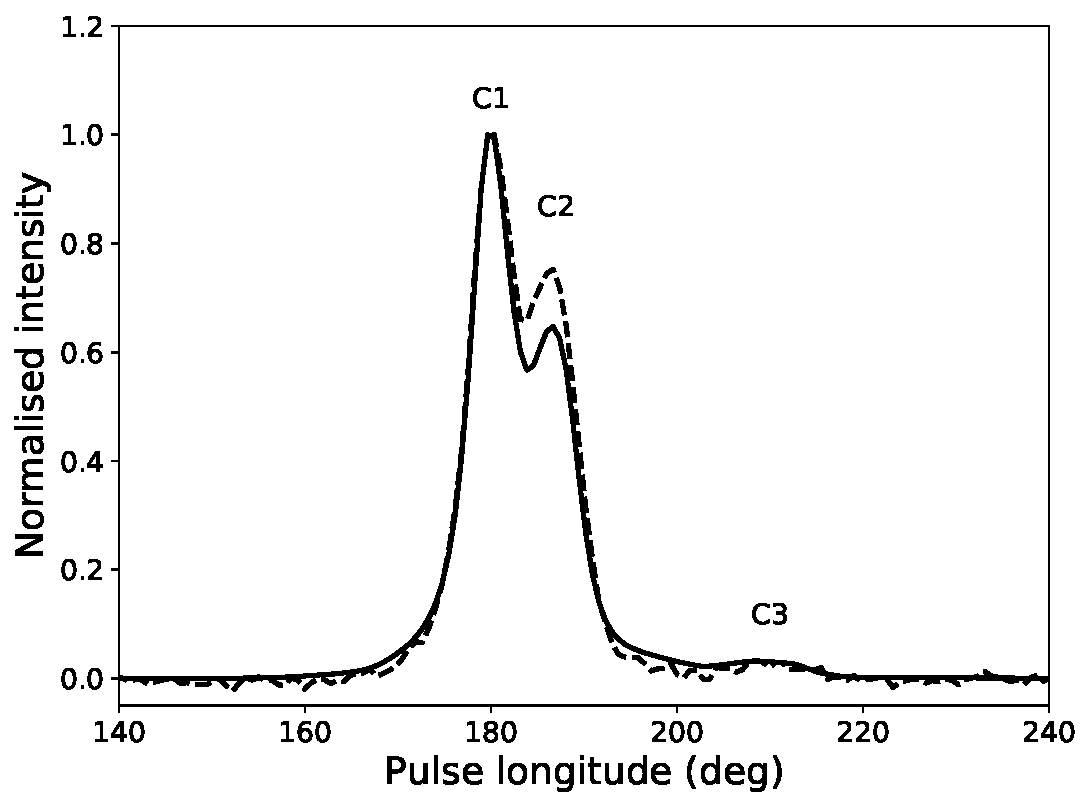
\includegraphics[width=0.6\textwidth]{Figures/J1518/profile_comparison}
        \caption[Profile comparison]{A comparison of the profile of PSR~J1518+4904 at 1250~MHz (solid line) with an archival profile at 1410~MHz \citep[dashed line,][]{KXL+1998}. Three main profile components are visible, labelled C1, C2, and C3 respectively. The small differences between the FAST data and the archival data are likely mostly spectral evolution (see the middle panel of Fig.~\ref{fig: J1518 - profile frequency evolution}).}
        \label{fig: J1518 - profile comparison}
    \end{center}
\end{figure}
The FAST profile is shown by the solid line while the archival observation is shown by the dashed line. Both profiles are normalised to their peak intensities, and are aligned by performing a cross-correlation using the \texttt{pmod} tool in \textsc{psrsalsa}. The pulse longitude range is cropped to show the detail of the main profile and its three components, C1, C2, and C3, which are labelled accordingly. There is little difference in the shape of the profiles, which indicates that we are safe to treat the FAST observation as though it is Stokes $I$. The slight difference in the relative intensity of component C2 could be entirely because of the difference in frequency of the two observations, as the profile does evolve with frequency as shown later in this section (the middle panel of Fig.~\ref{fig: J1518 - profile frequency evolution}).

\subsection{The pulse profile}
\label{sec: J1518 - analysis - new profile component}

The full-width integrated pulse profile of PSR~J1518+4904 is shown in the left-hand panel of Fig.~\ref{fig: J1518 - integrated profile}. The three observations which are unaffected by RFI are plotted together, with 2018-07-22 represented by the black line, 2018-08-04 the blue line, and 2018-11-04 the red line. The 2018-11-04 profile was aligned such that its peak lies at a longitude of $180\degr$. As it has the highest S/N, this profile was then used as a template to align the other two profiles by cross-correlation. All three profiles were normalised to a peak intensity of unity to aid visual comparison. No absolute flux calibration was possible for these commissioning data.
\begin{figure}
    \begin{center}
        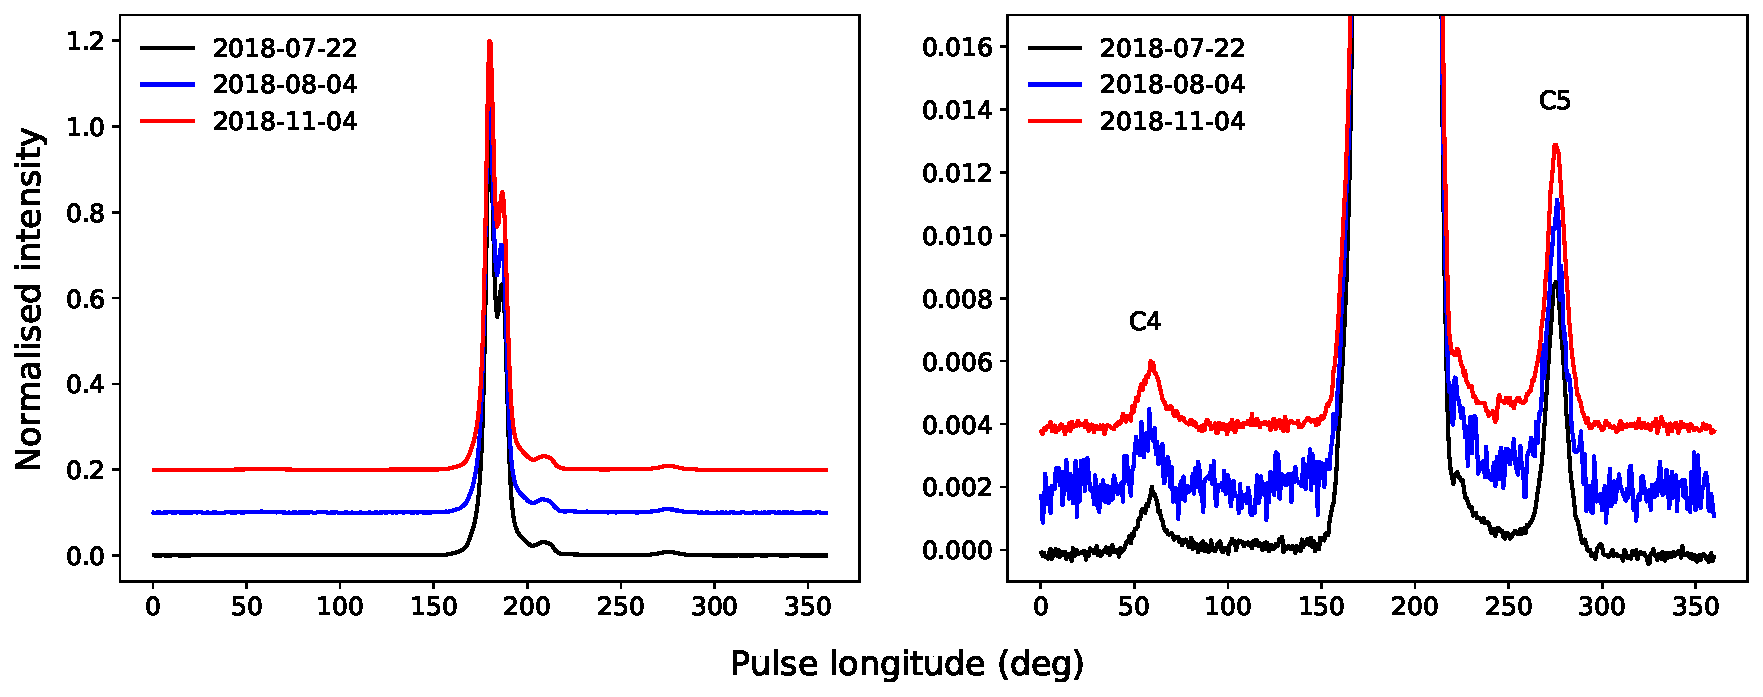
\includegraphics[width=1.0\textwidth]{Figures/J1518/profile_components}
        \caption[New profile components in PSR~J1518+4904]{(LEFT) The normalised profile of PSR~J1518+4904 (integrated over time and frequency) as observed at three different epochs, as indicated by the line colour. (RIGHT) The same profiles, but cropped to low intensities in order to highlight the weak profile components around $55\degr$ and $275\degr$ in pulse longitude, labelled C4 and C5 respectively. To aid comparison the different observations have been plotted with small vertical offsets.}
        \label{fig: J1518 - integrated profile}
    \end{center}
\end{figure}

The excellent sensitivity of FAST means that two new profile components could be identified. They are significantly weaker than the main component, around 0.9 and 0.2~per~cent respectively of the peak amplitude. The right-hand panel of Fig.~\ref{fig: J1518 - integrated profile} shows the same set of profiles as the left-hand panel, but cropped to one~per~cent of the peak intensity to highlight the newly identified components. The weaker of the new components is centred on $\sim$59$\degr$ pulse longitude, whilst the stronger lies at $275\degr$. This second new component is clearly connected to the main profile via a weak bridge of emission, while this is less clear for the weakest component. Both new components appear in all three observations with the same relative amplitude to the main peak, so they are confirmed to be stable profile features across a period of at least four months. The new leading component is too weak for it to be identified in the single-pulse data, but the new trailing component is faintly detectable.

\begin{figure}
    \begin{center}
        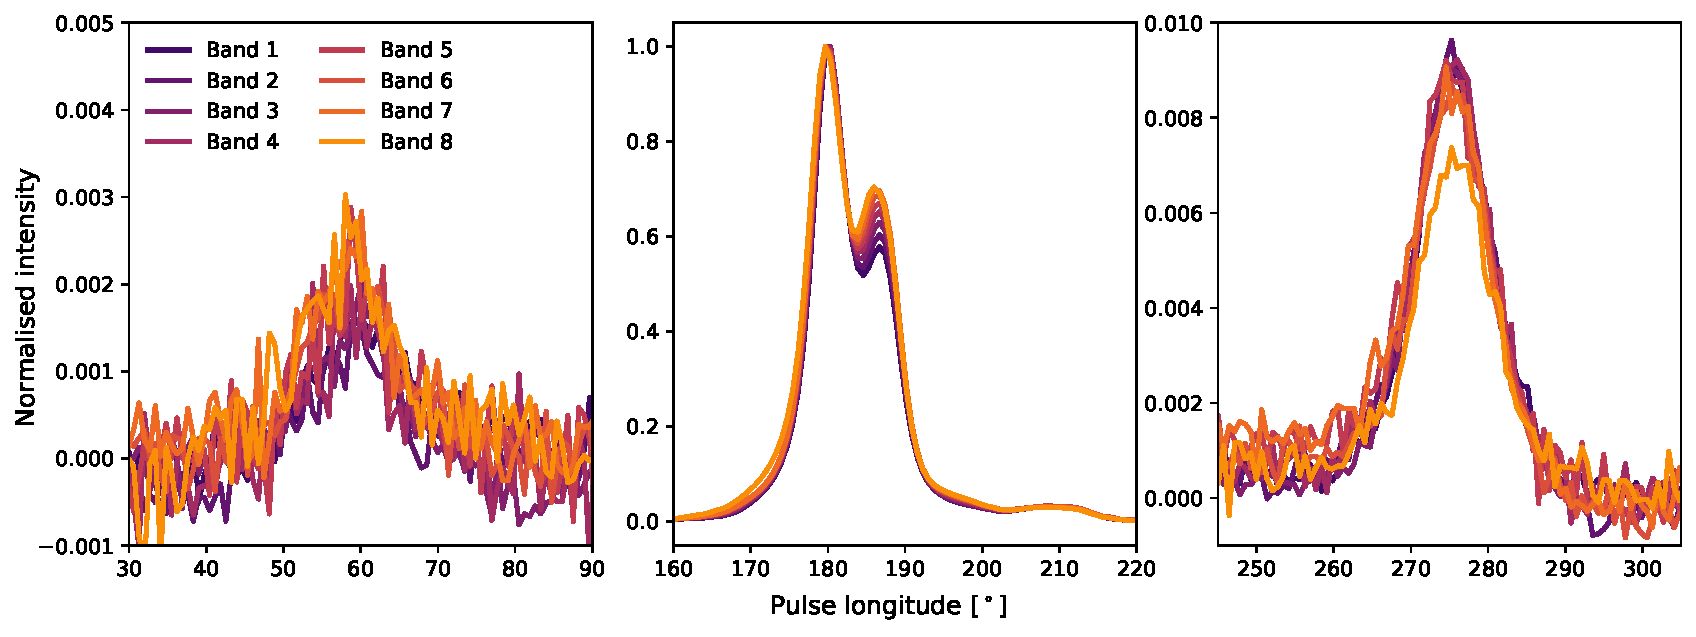
\includegraphics[width=1.0\textwidth]{Figures/J1518/profile_freq_evolution}
        \caption[Frequency evolution of profile components]{The frequency evolution of the three profile components across the eight sub-bands of the 2018-11-04 observation, shown here because it has the highest S/N profile due to its increased length -- the 2018-07-22 and 2018-08-04 observations are consistent. The weaker new component is shown in the left-hand panel (cropped to 0.5~per~cent of the main peak intensity to show the component more clearly). The main profile components are shown in the middle panel -- all eight sub-bands were normalised with respect to the amplitude of the main peak. The stronger new component at later pulse longitudes is shown in the right-hand panel. Neither of the new components appear to significantly change with frequency, but the intensity of the secondary peak of the main component gradually increases with frequency compared to the main peak.}
        \label{fig: J1518 - profile frequency evolution}
    \end{center}
\end{figure}

As illustrated by Fig.~\ref{fig: J1518 - profile frequency evolution}, the shape and relative amplitude of the new components are also stable across the 500~MHz frequency range covered by these observations. This figure shows a close-up view of the weak new component (left-hand panel), the main profile (centre panel), and the stronger new component (right-hand panel) across all eight frequency sub-bands in the 2018-11-04 observation. These are plotted in order of increasing frequency, in the colour gradient from deep purple to light orange. The weak new component appears relatively stable, and shows a possible slight increase in intensity with increasing frequency, but this is not significant. Similarly, the stronger new component (right-hand panel) appears unchanged across the frequency range, with the exception of band 8 (lightest orange) which appears attenuated. This suggests a rapid profile evolution starting to take place at the top end of the frequency range covered.

In the main profile (middle panel of Fig.~\ref{fig: J1518 - profile frequency evolution}), at least three distinct components are visible. The profiles are normalised to the leading, brightest, component ($180\degr$) so its frequency evolution is by definition removed. The weakest, trailing, component ($\sim$210$\degr$) does not appear to evolve with frequency. However, the middle component ($\sim$187$\degr$) appears to increase in intensity with increasing frequency relative to the main peak by a factor of approximately 1.3. The wings of the main peak (around $170\degr$ and $195\degr$) also show a slight trend of broadening with frequency. In all three panels, there is no indication that the peaks shift relative to one another in longitude with frequency, so the overall width and structure of the profile remains constant across the bandwidth. 

It should be stressed that because the profiles are normalised to the peak of the profile, only \textit{relative} changes can be detected. Also, because the data is not polarisation-calibrated, the shape of the profile could be somewhat distorted. It can not be ruled out that some of the frequency dependence in the profile shape is related to Faraday rotation. The linear and circular polarisation fractions are approximately 20~per~cent at 1410~MHz \citep{XKJ+1998}, with the (left-handed) circularly polarised emission associated with profile component C1, and the linearly polarised emission with profile component C2. The rotation measure of PSR~J1518+4904 is RM $= -15.6 \pm 3.7$~rad~m$^{-2}$ \citep{NPN+2020}, which means that the expected change in position angle $\Delta\psi \approx 45\degr$ across the observed bandwidth (see Sec.~\ref{sec: intro - observation processing - ISM effects - faraday rotation}), so Faraday rotation will be important to correct when studying the polarisation properties of this pulsar with FAST.

However, given the consistency of the different observations, in combination with the fact that this source is known to have only a modest degree of polarisation, this suggests that the main effect is profile evolution in Stokes $I$. The stronger new profile component extends the main profile width of PSR~J1518+4904 by a factor of $\sim$4, whilst the weaker one is sufficiently separated to be consistent with an interpulse. This new profile structure and its implications are discussed in Sec.~\ref{sec: J1518 - discussion}.








\subsection{Longitude-resolved fluctuation spectrum, LRFS}
\label{sec: J1518 - analysis - LRFS}

% \begin{wrapfigure}[20]{o}{0.4\textwidth}
\begin{figure}
    \begin{center}
        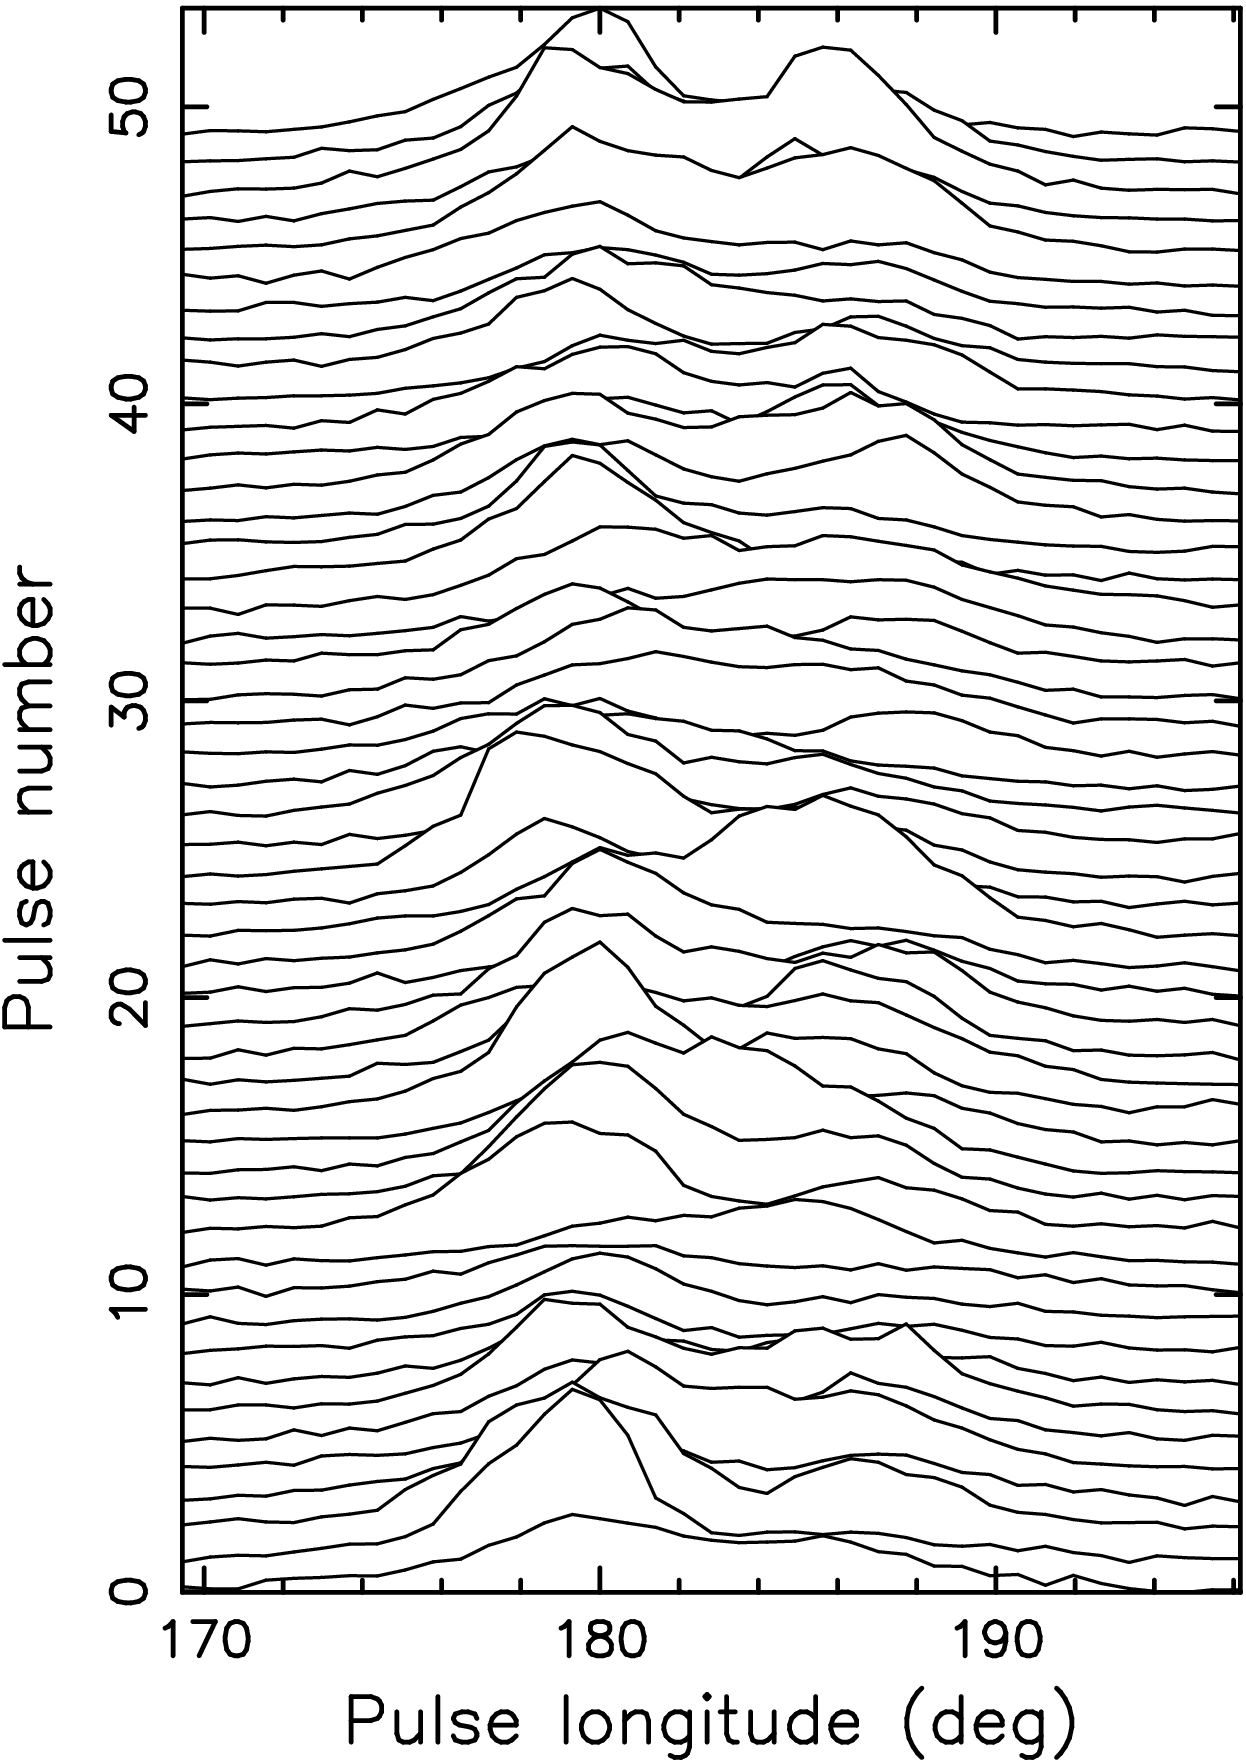
\includegraphics[width=0.4\textwidth]{Figures/J1518/stack_joy.png}
        \caption[Single pulses of PSR~J1518+4904]{A short stack of 50 pulses of PSR~J1518+4904 as observed with FAST on 2018-11-04 to illustrate how well the single pulses can be seen. Subpulse drift is occurring, but too rapidly for distinct driftbands to be resolved.}
        \label{fig: J1518 - short stack}
    \end{center}
\end{figure}
% \end{wrapfigure}
In contrast to previous studies of PSR~J1518+4904, our observations with FAST with its exceptional gain are sensitive enough to clearly detect single pulses, which means that fluctuation analysis of this MSP is possible in unprecedented detail. The quality of our data is illustrated in Fig.~\ref{fig: J1518 - short stack} which shows a short sequence of individual pulses cropped to focus on the main peak.

A longitude-resolved fluctuation spectrum (LRFS) was produced for each of the three analysed observations according to the method detailed in Sec.~\ref{sec: J1926 - analysis - single pulse variability}. The length of the Fourier transform used to calculate the LRFS was 1024 pulses, and all pulses were used for each epoch. Figure~\ref{fig: J1518 - lrfs time evolution} shows a magnified view of two pulse longitude regions of the LRFS for each observation.
The left-hand panels show the LRFS between longitudes $176\degr$ and $190\degr$ (covering profile components C1 and C2) whilst the right-hand panels show the region between $192\degr$ and $212\degr$ (between profile components C2 and C3). No significant periodic modulation was detected in the regions occupied by the new profile components. Although the two columns in the figure form a continuous longitude range, they are separated to allow the weaker spectral features at later longitudes to stand out better by having different dynamic ranges in the two sets of plots. The 2018-07-22 observation is shown in the top two panels, 2018-08-04 in the middle row, and 2018-11-04 in the bottom row. Each of the six plots is accompanied by a side panel (line plot) which shows the integrated power spectrum over the displayed longitude range.

\begin{figure}
    \begin{center}
        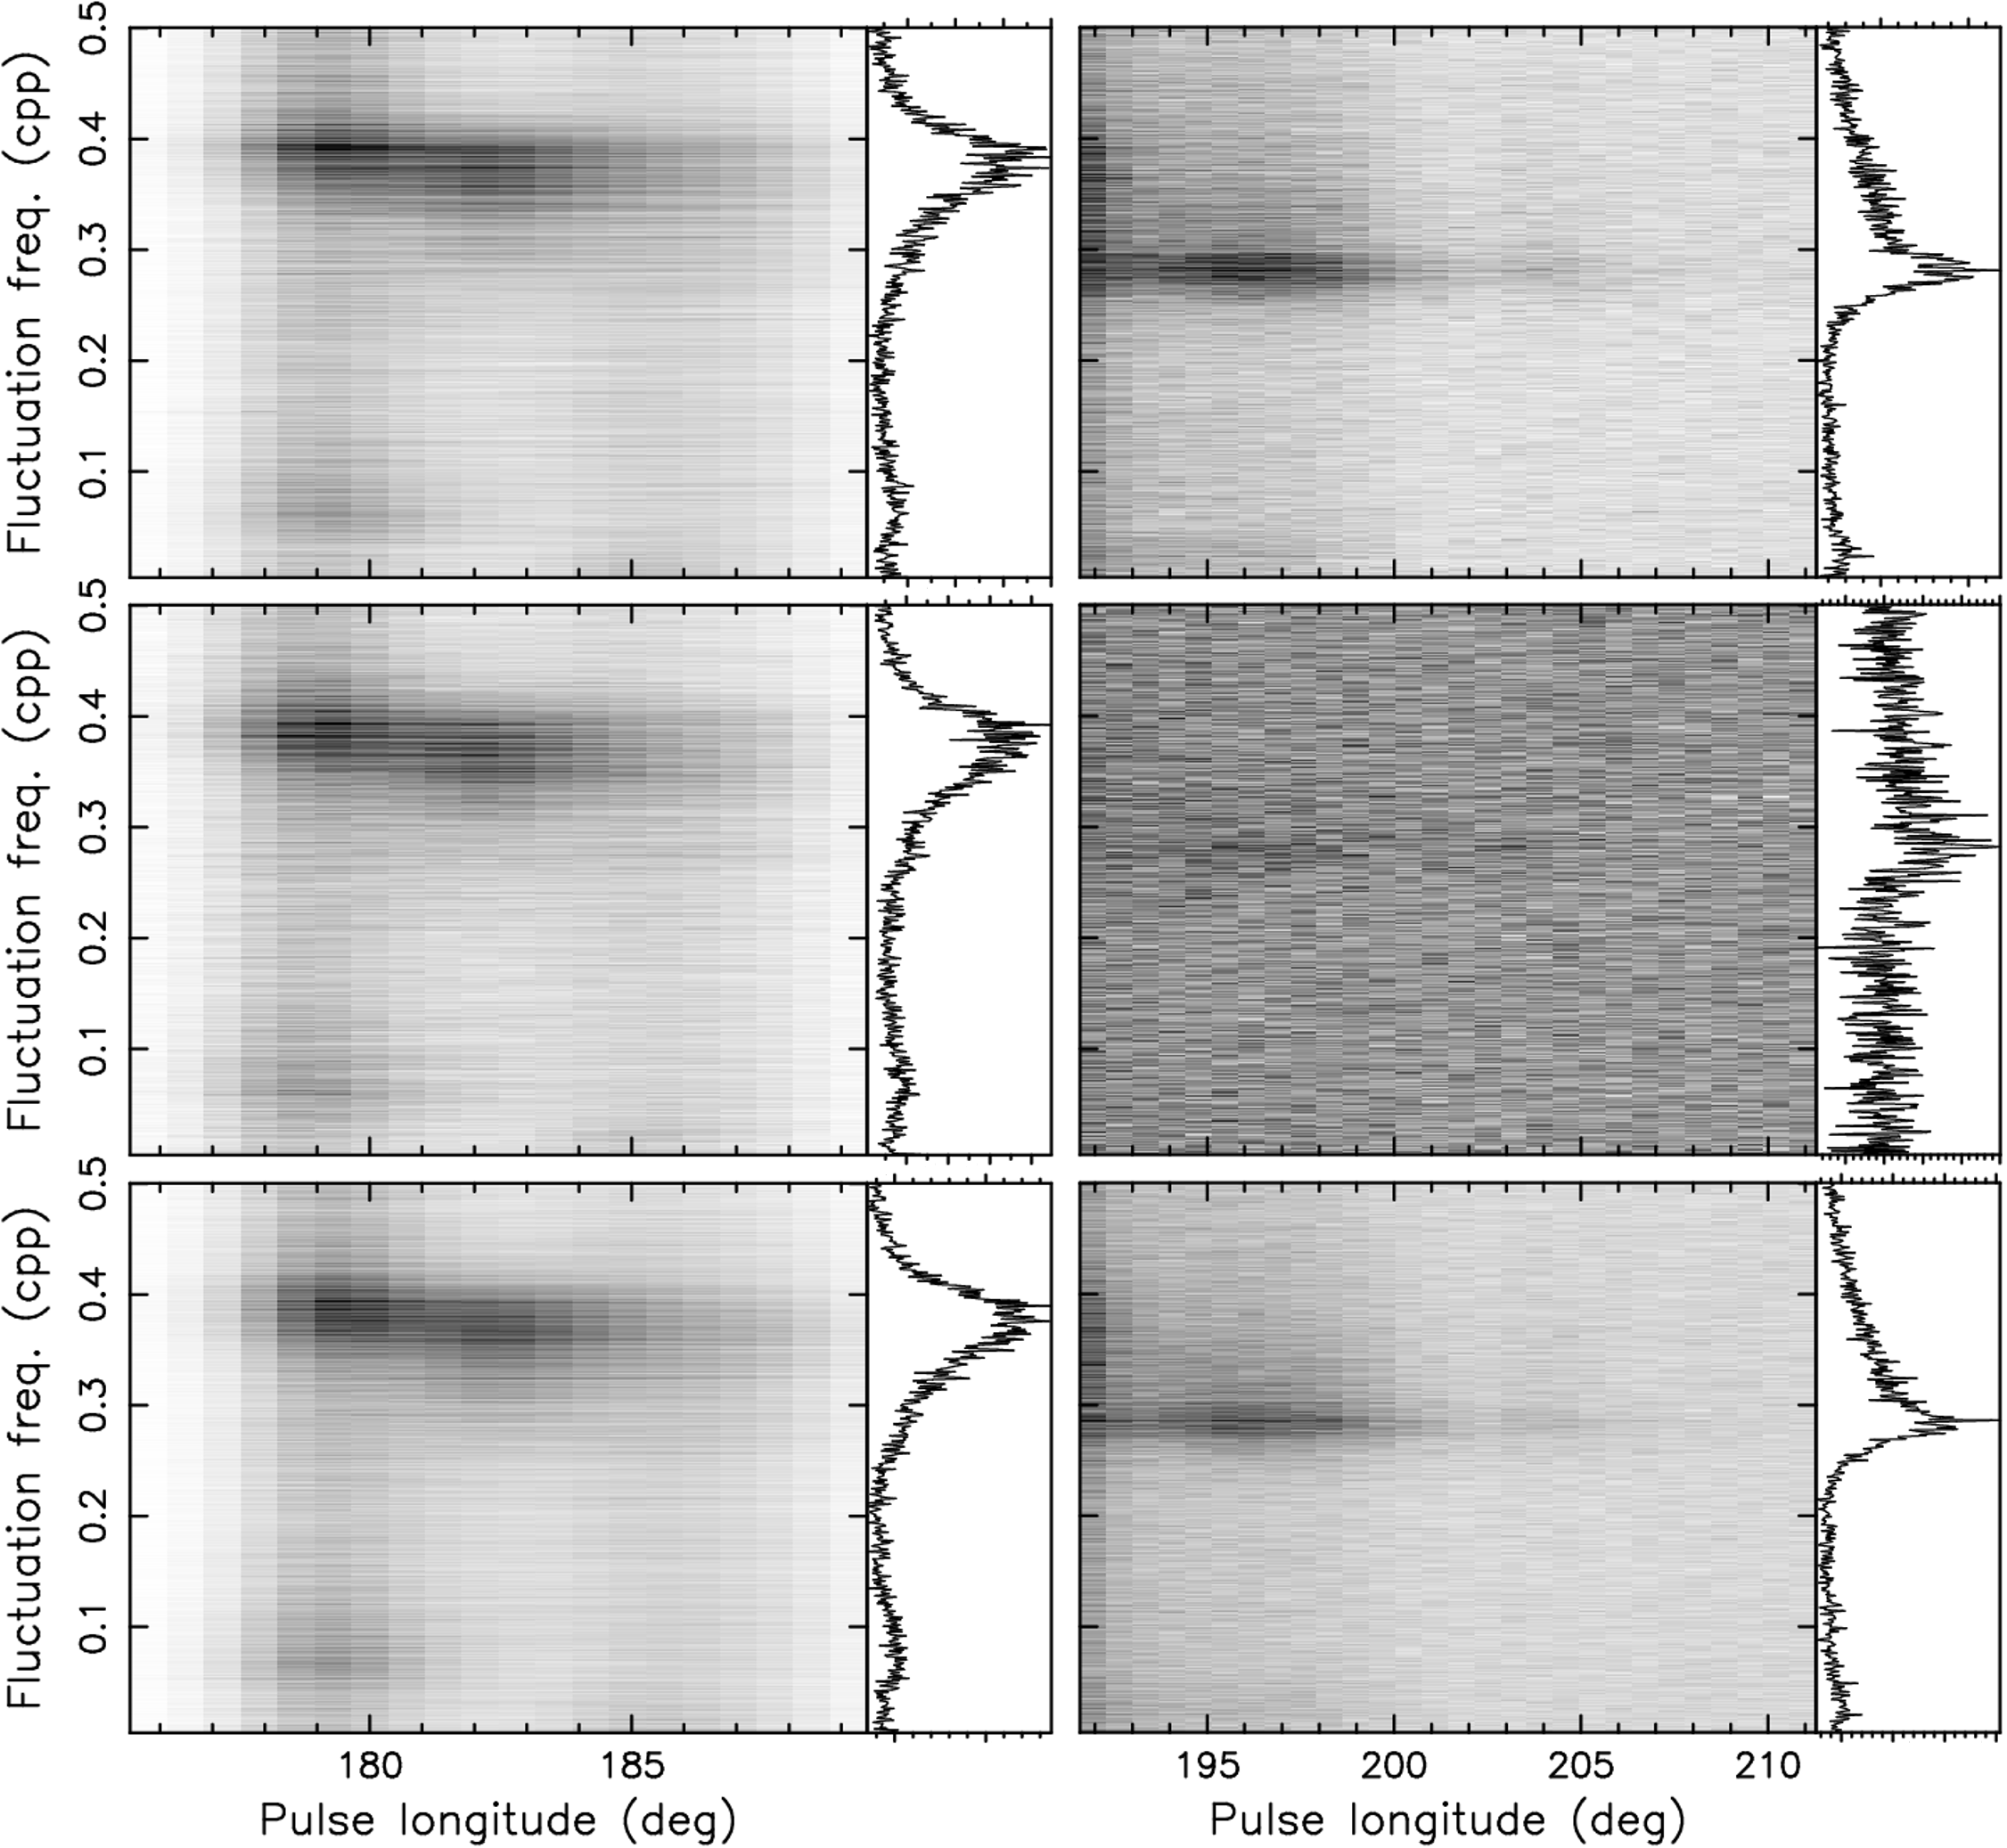
\includegraphics[width=1.0\textwidth]{Figures/J1518/lrfs_time_evolution_2}
        \caption[Longitude-resolved fluctuation spectra of PSR~J1518+4904]{The LRFS of PSR~J1518+4904 at three different epochs: 2018-07-22 (top row), 2018-08-04 (middle row), and 2018-11-04 (bottom row). The left-hand panels show the power spectrum between pulse longitudes $176\degr$ and $190\degr$, whilst the right-hand panels show the spectrum between longitudes $192\degr$ and $212\degr$. The fluctuation power in the earlier pulse longitudes strongly dominates that of the later longitudes, so they are shown separately. Two $P_3$ features are seen in the left-hand panels, the strongest peaking around 0.38~cpp and a fainter peak at around 0.07~cpp which is constrained to profile component C1. The spectrum of the later longitudes exhibits a single distinct $P_3$ peak at $\sim$0.29~cpp which appears in all three epochs (albeit only faintly in 2018-08-04).}
        \label{fig: J1518 - lrfs time evolution}
    \end{center}
\end{figure}

The left-hand panels show a very strong, broad spectral feature peaking at around 0.38 cycles per period (cpp) which extends across the displayed pulse longitude range. It covers the two brightest profile components, seen most clearly in the central panel of Fig.~\ref{fig: J1518 - profile frequency evolution}. There is a second, fainter spectral feature which is strongest between $178\degr$ and $180\degr$ pulse longitude and peaks at approximately $0.07$~cpp. This longer-period modulation appears to be localised within the brightest component C1 of the main peak of the profile. The features in the left-hand panels of Fig.~\ref{fig: J1518 - lrfs time evolution} are both quite broad in $P_3$, which indicates that although the pulse-to-pulse variability is periodic, the periodicity is somewhat irregular.

The right-hand panels of Fig.~\ref{fig: J1518 - lrfs time evolution} show the section of the LRFS that covers the longitude range occupied by the trailing shoulder of the main profile. The 2018-07-22 and 2018-11-04 observations (top and bottom panels) both show a somewhat more well-defined peak at around 0.28~cpp. The peak is quite asymmetric, with a long tail towards 0.5~cpp. This is best seen at the early side of the longitude range. The peak is also faintly visible in the 2018-08-04 observation (middle panel). This observation has a significantly lower signal-to-noise ratio than the other two (see the right hand panel of Fig.~\ref{fig: J1518 - lrfs time evolution}). Nevertheless, compared to the periodic modulation at earlier longitudes (left-hand panel), it seems that the 0.28~cpp modulation is significantly weaker during this epoch without the overall relative intensity of the profile at this pulse longitude range being affected (see Fig.~\ref{fig: J1518 - integrated profile}).

Although they are connected in pulse longitude, the periodicities in the pulse-to-pulse modulation are distinctly different in the two regions. In addition, the periodicity seems to shift with pulse longitude in the left-hand panels as well. This will be described and discussed further in Sec.~\ref{sec: J1518 - discussion - funky P3}.
Figure~\ref{fig: J1518 - lrfs time evolution} shows that the main features in the LRFS of PSR~J1518+4904 are stable over the period over which the different observations took place. In order to investigate the stability of the features as a function of frequency, the LRFS was explored for the eight sub-bands of the 2018-11-04 observation. These results are shown in Fig.~\ref{fig: J1518 - lrfs freq evolution}, which are similar to Fig.~\ref{fig: J1518 - lrfs time evolution}, except that two panels are shown per frequency sub-band (the sub-band label is shown in the top-left of each panel in the first and third columns). It is evident that the main features of the LRFS are independent of frequency. This is a general property of drifting subpulses, where the periodicity $P_3$ is observed to be independent of frequency \citep{WSEx2007}. It also rules out that these spectral features are because of incidental narrowband RFI (although the fact that the features are not found in the off-pulse region also rules that out).




\begin{landscape}
    \begin{figure}
        \begin{center}
            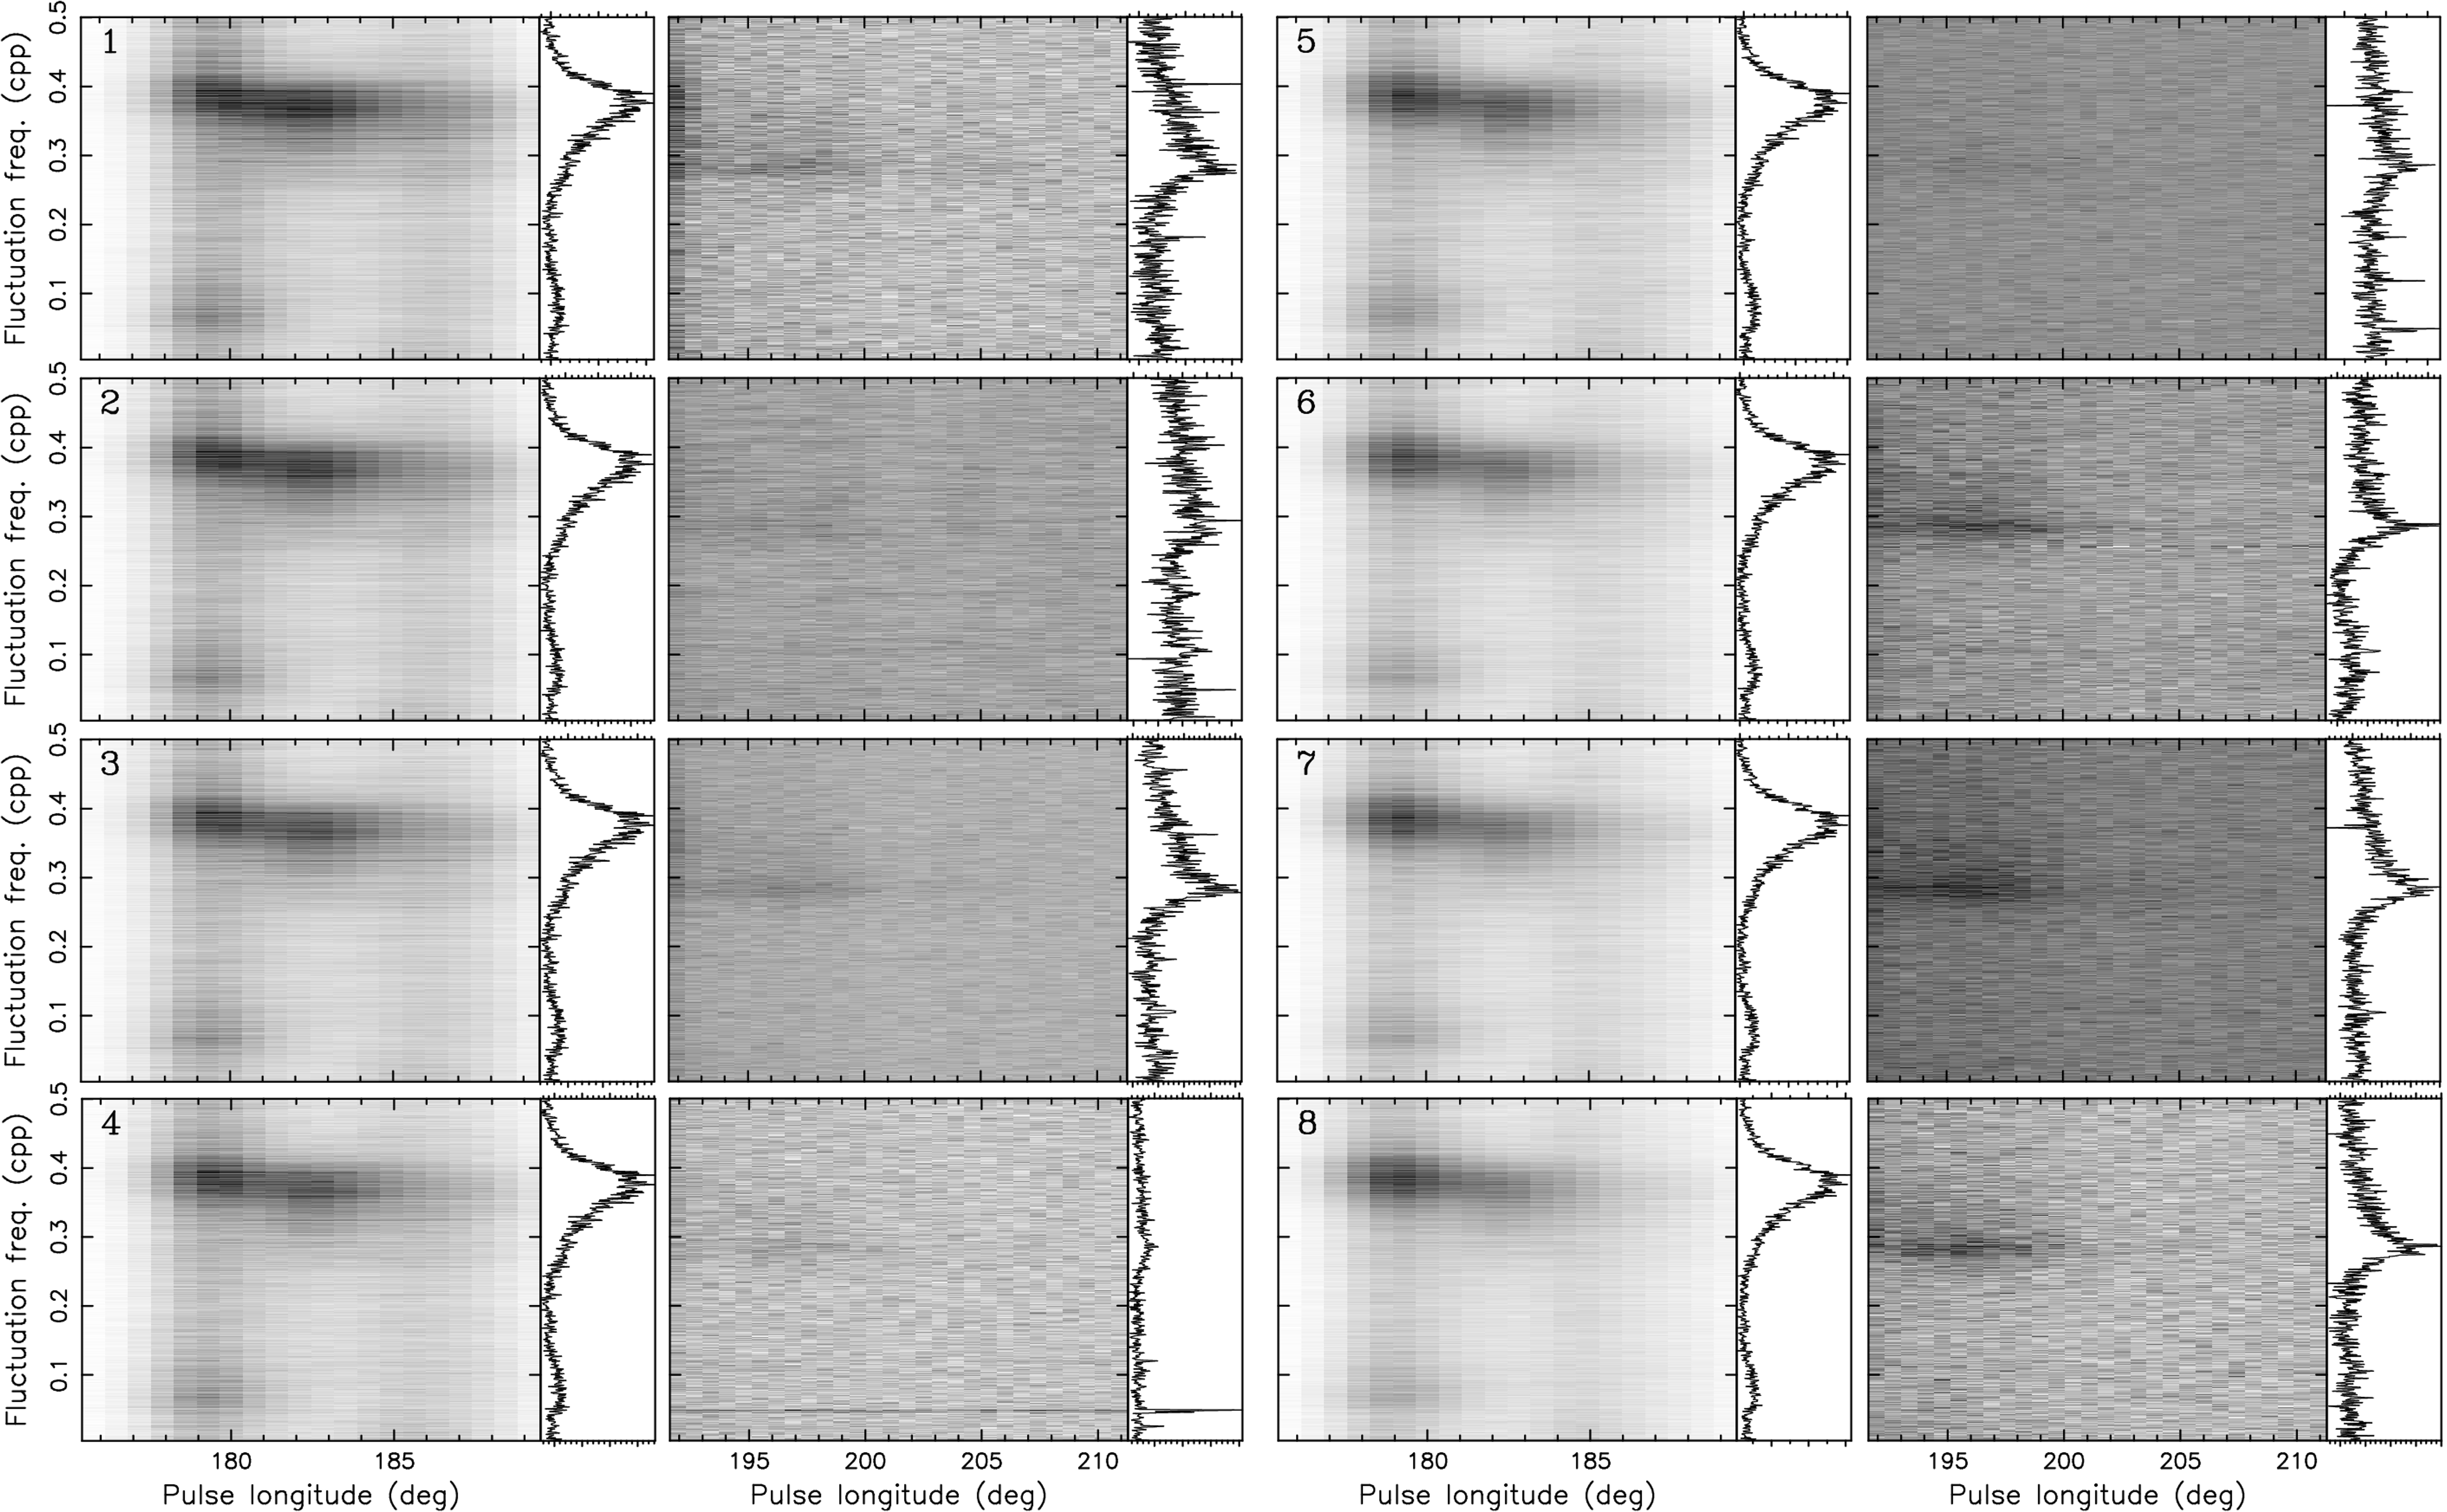
\includegraphics[width=0.82\textheight]{Figures/J1518/lrfs_freq_evolution_2}
            \caption[Frequency evolution of the LRFS]{The frequency evolution of the two components of the LRFS across the 2018-11-04 observation, where the two panels per frequency band are as described in Fig.~\ref{fig: J1518 - lrfs time evolution}. The frequency band number is shown in the top-left corner of panels corresponding to the spectrum of the main component. The frequencies covered by the sub-bands are defined in Table~\ref{tab: J1518 - frequency sub-bands}. Frequency increases with sub-band number. The main features of the LRFS are visible across the full frequency range.}
            \label{fig: J1518 - lrfs freq evolution}
        \end{center}
    \end{figure}
\end{landscape}




\subsection{Two-dimensional fluctuation spectrum, 2DFS}
\label{sec: J1518 - analysis - 2DFS}
\begin{figure}
    \begin{center}
        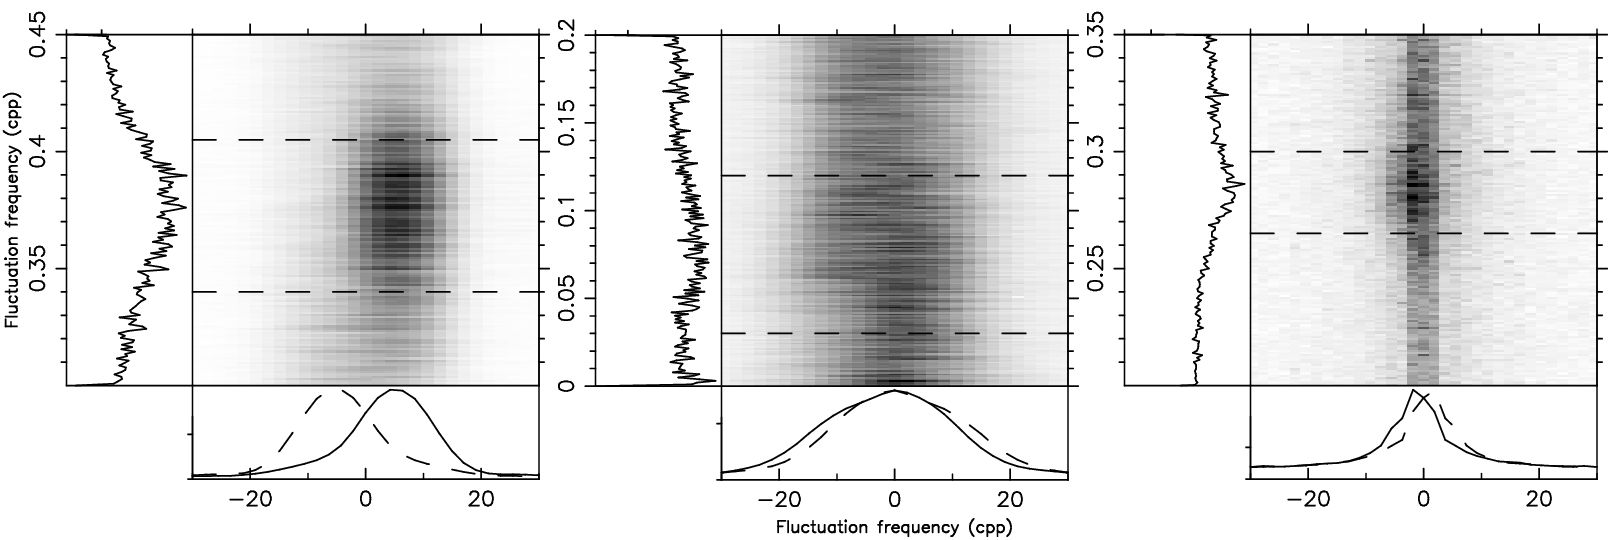
\includegraphics[width=\textwidth]{Figures/J1518/2DFS_all}
        \caption[2DFS of PSR~J1518+4904]{The 2DFS of PSR~J1518+4904, calculated from the 2018-11-04 observation. The left-hand and middle panels were calculated using a pulse longitude range of $102\degr$ to $191\degr$ (enclosing profile components C1 and C2), and the right-hand panel used longitudes from $194\degr$ to $1283\degr$ (C3). The shading shows the power at a given $P_1/P_2$ ($x$-axis) and $P_1/P_3$ ($y$-axis) fluctuation frequency, with more power shown as darker grey. The line plot to the side of each panel shows the $P_1/P_3$ distribution integrated horizontally across the window, and the solid lines in the line plots below show the $P_1/P_2$ distribution integrated vertically between the horizontal dashed lines. The dashed line in the lower line plots shows the $P_1/P_2$ distribution reflected about $P_1/P_2 = 0$ to highlight any asymmetry.}
        \label{fig: J1518 - 2DFS}
    \end{center}
\end{figure}

A 2DFS as described in Sec.~\ref{sec: J1926 - analysis - single pulse variability} was created for PSR~J1518+4904, using the 2018-11-04 observation. Unlike the LRFS, which is only sensitive to fluctuation periodicities from pulse to pulse ($P_3$), the 2DFS is also sensitive to longitudinal drift associated with these periodicities ($P_2$). Figure~\ref{fig: J1518 - 2DFS} shows the 2DFS calculated for the three features seen in the LRFS, at 0.38~cpp (left panel), 0.07~cpp (centre panel) and 0.28~cpp (right panel) respectively. The three panels have been cropped to show the $P_3$ range of interest for each feature: the line plots in the panels to the left of each plot show the integrated $P_3$ power spectrum, and the solid line plots beneath each plot show the $P_2$ power spectrum integrated between the horizontal dashed lines which delimit the location of the features in $P_3$. The dashed lines in the same panels show the integrated $P_2$ peak reflected about $P_1/P_2 = 0$~cpp in order to highlight any asymmetry.

Using the \texttt{pspecDetect} tool in \textsc{psrsalsa}, the position of the features in the 2DFS were quantified. For the 0.38~cpp feature, the centroid is located at $P_2 = 69\degr \pm 1 \degr$, and $P_3 = 2.660 \pm 0.005\ P_1$. The centroid of the 0.28~cpp feature is at $P_2 = -250\degr \pm 40 \degr$, and $P_3 = 3.51 \pm0.02\ P_1$. The 0.07~cpp feature in the middle panel is weak, without it standing out from the non-periodic modulation power in the 2DFS, but the asymmetry of its $P_2$ spectrum implies a slightly negative $P_2$, indicating drifting. The sign of $P_2$ indicates the direction of drift: a positive $P_2$ shows that subpulses are moving towards later longitudes, or from left to right across the profile. The drift rate is given by $D=P_2 / P_3$, so for the 0.38~cpp component $D=+25.9\pm0.4$~$\degr/P_1$, and for the 0.28~cpp component $D = -70 \pm 10$~$\degr/P_1$. Both of these are exceptionally rapid drift rates, implying the modulation is almost `longitude stationary', i.e. modulation where the driftbands are practically horizontal. The values of $P_1/P_2 = 10$~cpp and $P_1/P_3 = 0.38$~cpp were previously determined by \citet{ESxx2003} (see Sec.~\ref{sec: J1518 - intro}) -- their value of $P_2$ differs from our own, possibly because they use the full pulse profile in their calculation (whereas we separate the components with different periodicities) which could effectively average $P_2$ of the different components and reduce the apparent drift rate. 

The periodic modulation is relatively imprecise, and because of the additional non-periodic modulation, the drifting subpulses are difficult to recognise in a pulse stack (see Fig.~\ref{fig: J1518 - short stack}). However, they are clearly detected in the statistical analysis such as with the 2DFS. It is exceptional that the  drift features are moving in opposite directions (they have different signs of $P_2$), especially in the same component. This will be further discussed in Sec.~\ref{sec: J1518 - discussion - funky P3}.















\subsection{Longitude-dependence of \texorpdfstring{$P_3$}{P3}}
\label{sec: J1518 - analysis - drifting P3}
\begin{figure}
    \begin{center}
        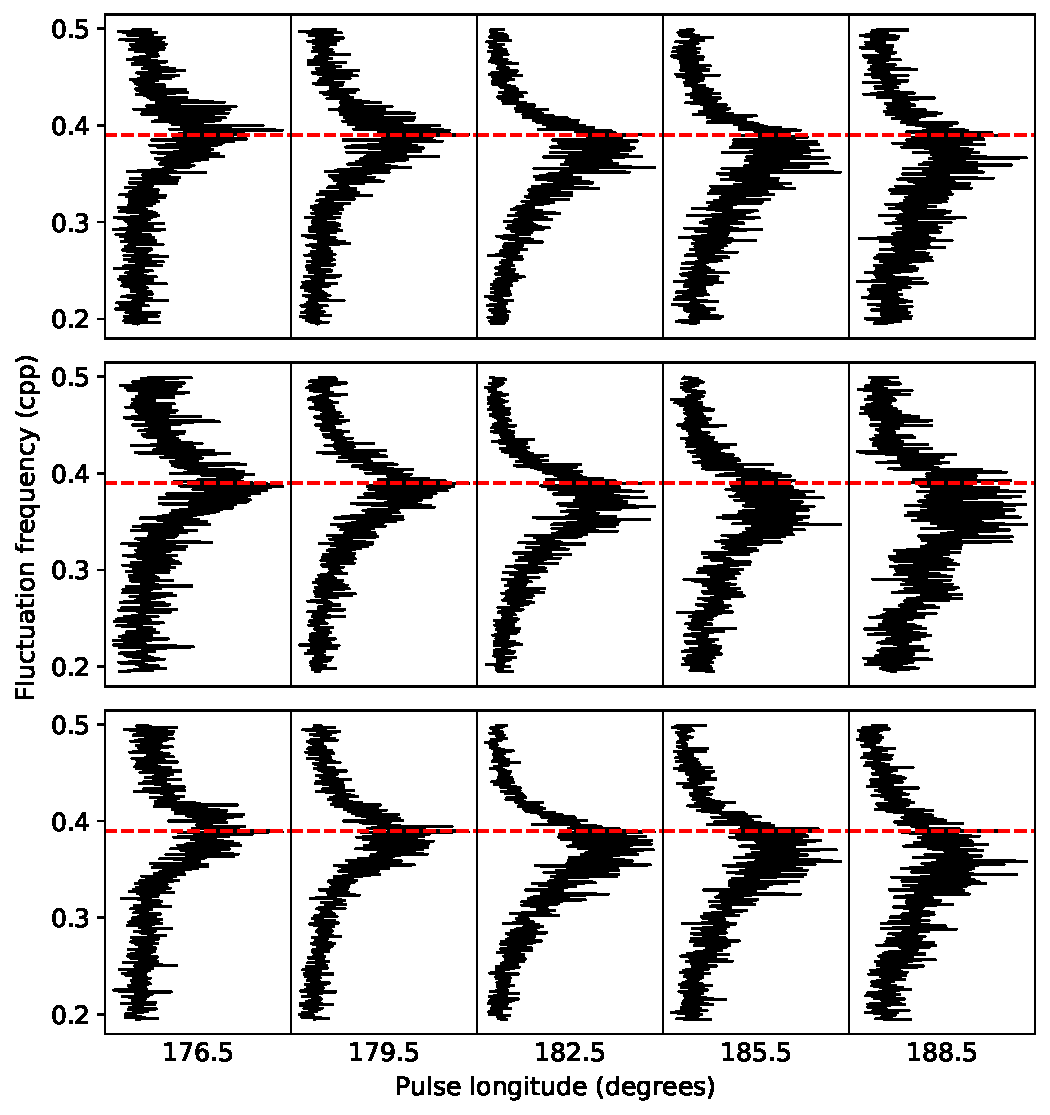
\includegraphics[width=0.55\textwidth]{Figures/J1518/drifting_P3}
        \caption[Drifting $P_3$ values in the main profile components]{The shift in the modulation frequency corresponding to $P_3$ across profile components C1 and C2, which is present in all epochs (top row -- 2018-07-22; middle row -- 2018-08-04; bottom row -- 2018-11-04). A range of pulse longitude of $15\degr$ between $175\degr$ and $190\degr$ was divided into $3\degr$ blocks, and the longitude-integrated LRFS (between 0.2 and 0.5~cpp) for each is shown from left to right (their central pulse longitude is shown on the $x$-axis). The red line indicates the peak of the earliest spectrum.}
        \label{fig: J1518 - drifting P3 components}
    \end{center}
\end{figure}

The dominant LRFS peak at $0.38$~cpp associated with profile components C1 and C2 appears to show a slight, but clear, evolution with pulse longitude, moving towards lower modulation frequencies as longitude increases while the spectral feature itself also becomes broader. This was investigated for all three epochs by dividing the LRFS into five blocks covering $3\degr$ in pulse longitude, between $175\degr$ and $190\degr$. These plots are shown in Fig.~\ref{fig: J1518 - drifting P3 components} -- as before, the top row shows the 2018-07-22 observation, the middle row is 2018-08-04, and the bottom row is 2018-11-04. All longitude bins across each $3\degr$-wide LRFS block were summed to produce the integrated spectra shown; their central pulse longitude is indicated on the $x$-axis. The displayed fluctuation frequencies have been limited to between 0.2 to 0.5~cpp in order to show the shift of the peak more clearly. This plot clearly demonstrates that the peak of the LRFS decreases in fluctuation frequency with increasing longitude by approximately $0.02$~cpp over the span, and this is the case for all three epochs. The red dashed line corresponds to a fluctuation frequency of 0.38~cpp, aligning with the peak of the spectrum at $176.5\degr$ (left-hand panels). The peak also becomes slightly broader with increasing longitude, and more noisy as a result of the decrease in spectral power with longitude. Overall, this seems to be part of a trend across the profile which ultimately leads to the modulation between profiles components C2 and C3 with a very different modulation period (0.28~cpp).  This is discussed further in Sec.~\ref{sec: J1518 - discussion - funky P3}.















\subsection{Evidence for disjoint drift modes}
\label{sec: J1518 - analysis - disjoint modes}

The existence of multiple discrete peaks in the LRFS as observed in other pulsars implies mode-switching, where the pulsar changes between different discrete drift states such that only one periodicity is visible at a given time in the pulse sequence. For example PSR~B0031$-$07 as described in Chapter~\ref{chapt: B0031} has three modes of drifting subpulses with modulation periods of $P_3 \approx 13P_1$, $P_3\approx 7P_1$ and $P_3 \approx 4P_1$ respectively. The pulsar abruptly switches between these modes. The modes have durations which have a characteristic timescale, but the distribution of durations is often broad. In addition, different profile components of pulsars are generally observed to share strictly identical periodicities. In PSR~J1518+4904 there are two discrete modulation periods in the leading component of the main peak (corresponding to 0.38 and 0.07~cpp). In addition, in the emission between components C2 and C3 a frequency corresponding to 0.28~cpp is present which is distinctly different from what is seen in the main pulse. Mode changes are known to occur with a wide range of timescales, typically on the order of minutes to hours, with the pulsar spending most of its time in the \textit{normal} mode and less frequently enters the \textit{abnormal} mode, with a distinctly different profile shape (e.g. \citealt{Sxxx2018} and references therein). Mode changing most commonly occurs in pulsars whose profiles comprise multiple components \citep{Rxxx1986}. The 2018-11-04 observation contains 88,400 single pulses, so there is certainly scope for two different drift modes occurring at different times to be present. The overarching question is if the different modulation periodicities occur simultaneously or if they are the result of mode changes. Since the LRFS is the average spectrum of the full observation, it cannot be used to distinguish between these two scenarios. 

Introduced by \citet{SSW+2009}, the sliding two-dimensional fluctuation spectrum (S2DFS) provides a way to study the time dependence of the fluctuation spectrum across the span of an observation. In this method fluctuation spectra are calculated as before, but with a slight difference. Instead of dividing the pulse stack up into equal-length blocks for which the power spectra are summed, the 2DFS is instead applied to a single window of $n$ pulses. The resulting spectrum is then collapsed in either the $P_2$ or $P_3$ direction, to create a one-dimensional spectrum for that block. The window of $n$ pulses is then shifted by one pulse and the process repeated. If the initial pulse stack consisted of $m$ pulses, then the result of the S2DFS is a `map' of $m-n+1$ collapsed spectra. This process allows any changes in the modulation to be resolved over timescales longer than $n$ pulses, the length of the discrete Fourier transform (DFT). A longer window can allow finer structures in the fluctuation spectra to be resolved, with the tradeoff of a reduced temporal resolution.

In this project, the individual fluctuation spectra were collapsed along the $P_2$ direction in order to attempt to resolve any evolution of $P_3$ during the observation. If PSR~J1518+4904 switches between drift modes with different periodicities on a timescale larger than the DFT size, then we can expect to observe spectral power alternating between distinct frequencies in the S2DFS. A DFT size of 256 pulses was chosen as a compromise between a sufficient spectral resolution without reducing the temporal resolution unnecessarily. Figure~\ref{fig: J1518 - S2DFS} shows a section of the S2DFS for the 2018-11-04 observation, over a span of 10,000 single pulses towards the end of the observation. This region was chosen because the pulsar was closer to the horizon at the start of the observation and its signal was weaker as a consequence, hence the modulation is less pronounced in earlier pulses. Nevertheless, this region is representative of what is observed over the full observation. The three panels show magnified regions of the S2DFS, which was computed for the three periodicities visible in the LRFS. The periodicity around 0.38~cpp is shown in the top panel, 0.28~cpp in the middle, and 0.07~cpp in the lower panel. The broadness (in frequency) of the spectral features in the in the LRFS can be understood as stochastic variability in the fluctuation frequency. The broad peaks in the right-hand side panels are the result of the addition of many narrow frequency features seen on short timescales. This variability seems erratic, with no resolved gradual systematic changes in the frequency as a function of time. Comparing the three panels, there is no evidence for switching such that only one of the main spectral features seen in the LRFS is visible at a given pulse-number interval. Therefore, the different modulation frequencies appear to be present at all times during the observation. The effect of the FFT length limiting the time resolution is evident -- one can see that the individual spectral features are smeared out slightly along the pulse number direction. If mode-switching happens on shorter timescales than the FFT length, it will not be resolved. So very rapid mode changes cannot be ruled out with this analysis.

\begin{figure}
    \begin{center}
        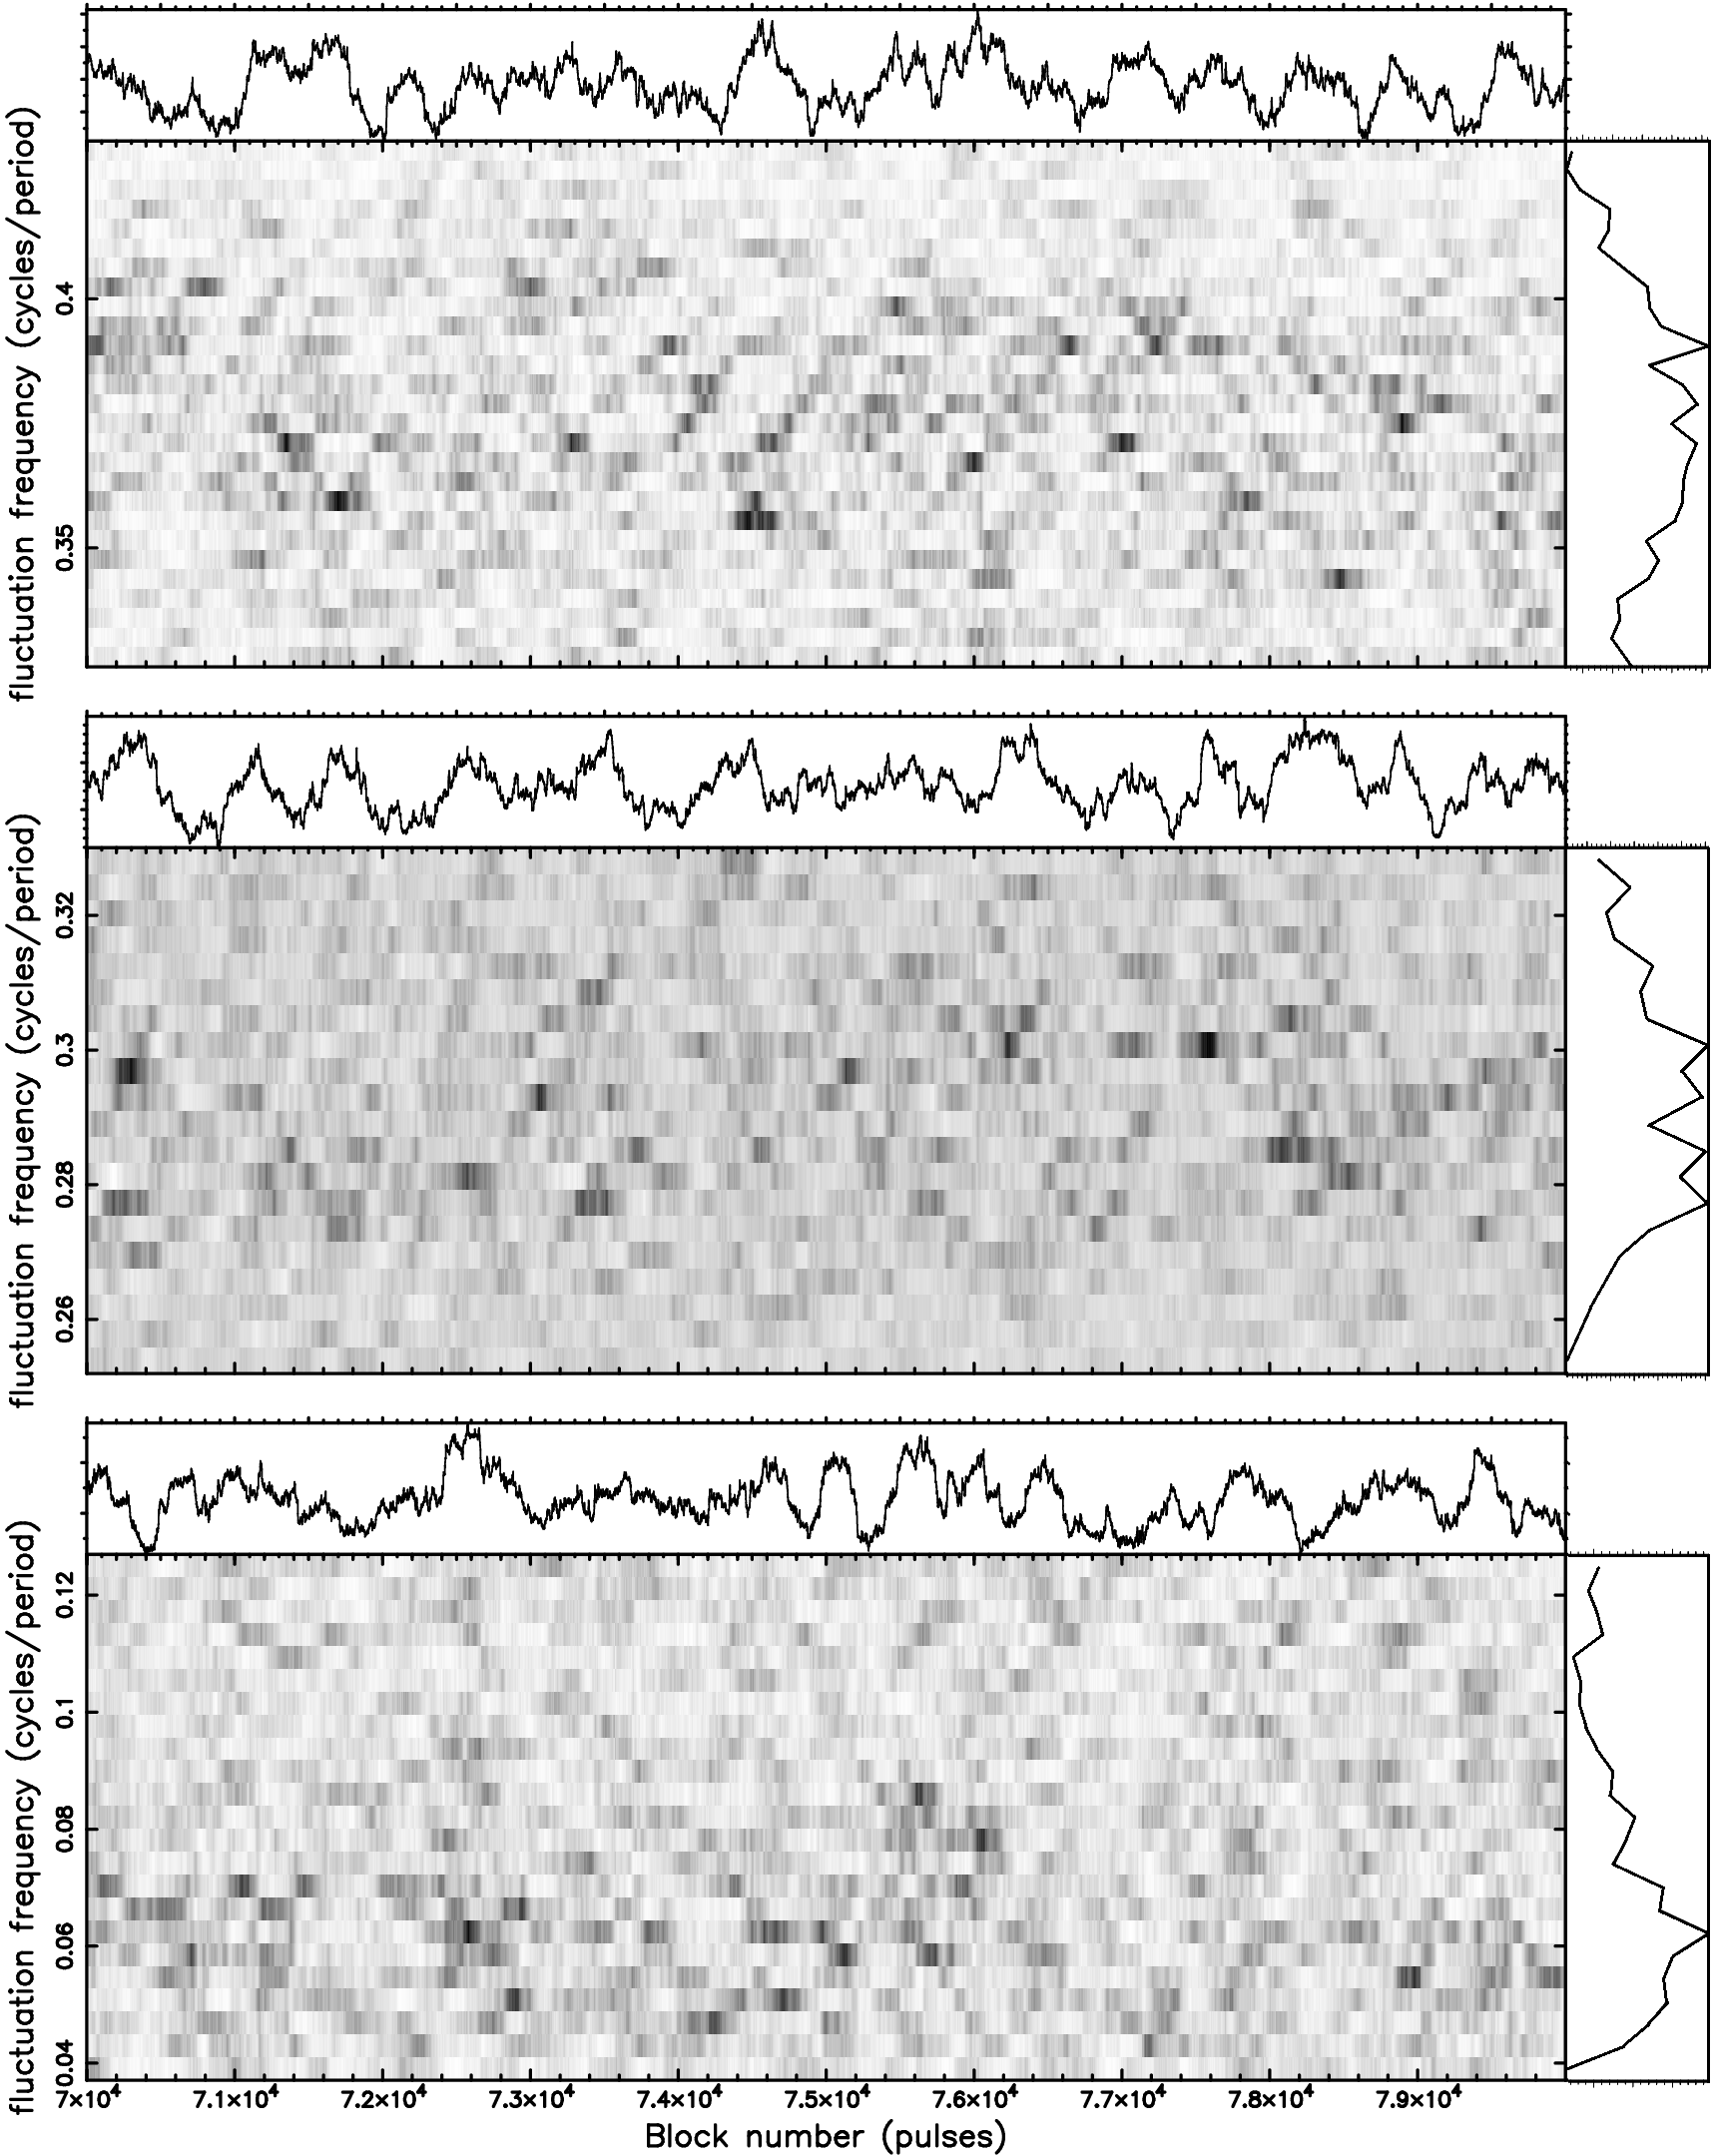
\includegraphics[width=1.0\textwidth]{Figures/J1518/S2DFS_256_2.png}
        \caption[The sliding 2DFS]{A section of the S2DFS for the 2018-11-04 observation, between pulse numbers 70,000 and 80,000. The three plots show different frequency ranges of the $P_3$ spectrum, cropped to show the feature at 0.38~cpp in the upper plot, 0.28~cpp in the middle, and 0.07~cpp in the lower panel. Alongside each greyscale plot, the top panel shows the total modulation power as a function of time, showing that $P_3$ varies stochastically within the envelope shown in the right-hand side panel. No mode switching is observed whereby only one of the three periodicities is seen at a given time.}
        \label{fig: J1518 - S2DFS}
    \end{center}
\end{figure}



As the S2DFS analysis proved inconclusive in showing the existence of distinct drift modes, an alternative method was explored. As shown by the LRFS (e.g. Fig.~\ref{fig: J1518 - lrfs time evolution}) the two $P_3$ features at 0.38~cpp and 0.28~cpp are associated with different pulse longitude ranges. In general drift mode changes are associated with changes in the shape of the average pulse profile. If this is the case in PSR~J1518+4904, then we might expect relative (correlated or anti-correlated) changes in intensity at the two distinct pulse longitude ranges. By calculating the flux density of the emission by integrating over the two ranges, we can look for a bimodality in a scatter plot of these two quantities.

\begin{figure}
    \begin{center}
        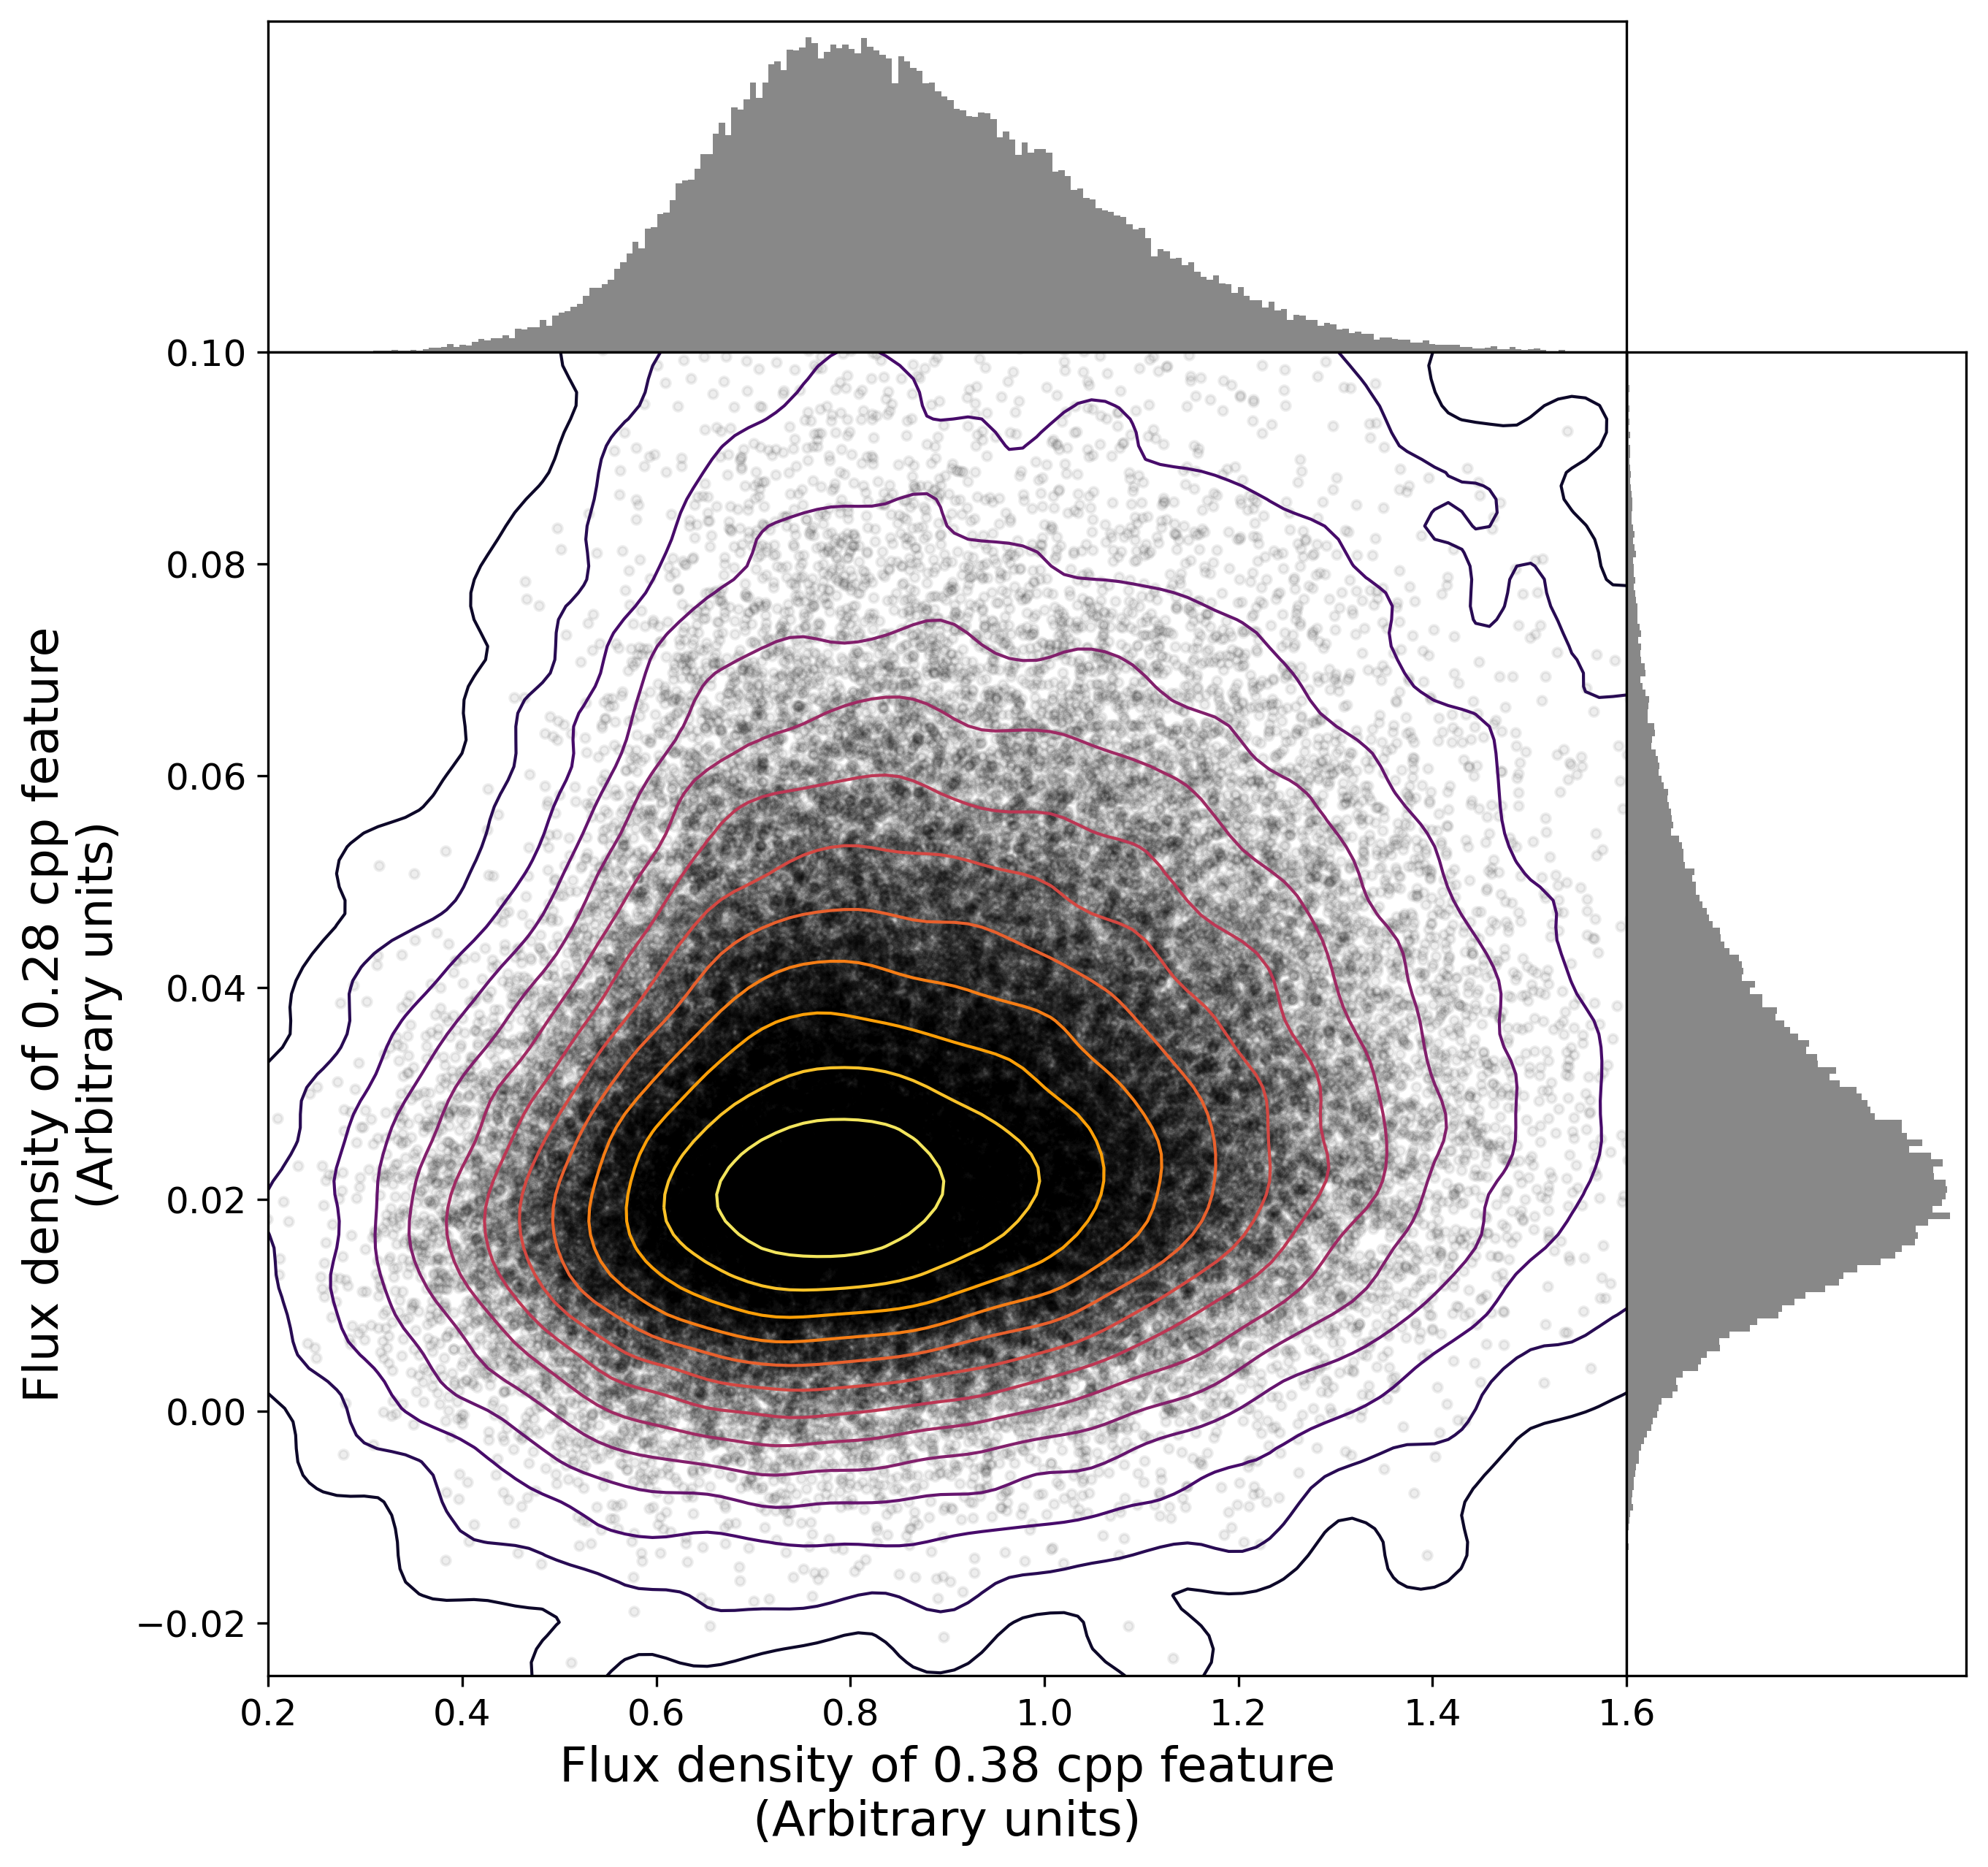
\includegraphics[width=0.7\textwidth]{Figures/J1518/energy_scatter.png}
        \caption[Profile component flux density comparison]{A scatter plot of the flux densities (in arbitrary units) integrated over the pulse longitude ranges corresponding to the modulation features at 0.38~cpp ($x$-axis) and 0.28~cpp ($y$-axis). The two quantities are shown in a scatter plot to highlight any correlation between them, after accounting for long-term variations in both components caused by the changing brightness of the pulsar over the course of the observation. The histograms in the side panels show the overall distribution for each pulse longitude range.}
        \label{fig: J1518 - energy scatter plots}
    \end{center}
\end{figure}

The flux densities integrated over the two pulse longitude ranges were measured using \texttt{penergy} in \textsc{psrsalsa} for all individual pulses, and these were then plotted against each other in a scatter plot. Long-term intensity variations caused by the changing elevation of the pulsar during the observation (and therefore its brightness) were removed by dividing the individual flux density measurements by the integrated flux density for the full profile using a running mean of 101 pulses. Figure~\ref{fig: J1518 - energy scatter plots} shows these results. The main panel shows the distribution in the relationship between the flux densities of the two regions, with the integrated flux density of the profile between $175.6\degr$ and $190.7\degr$ on the $x$-axis, and that of the region between $194.0\degr$ and $199.7\degr$ on the $y$-axis. Since the data is not flux-calibrated, these quantities are in non-physical units. The side panels show the overall integrated flux density distributions for the two regions. If mode-switching -- and hence an associated profile change where the relative intensity at the two pulse longitude regions is changing -- were occurring, we would expect bimodal structure with two distinct `islands' of points. No such feature can be seen in Figure~\ref{fig: J1518 - energy scatter plots}. If there is any bimodality in the flux density distribution, it is completely swamped by the pulse-to-pulse variability -- an attempt was made to account for this by summing every five pulses to smooth out short-term pulse shape changes associated with the periodic modulation. This had the effect that the distribution of points becomes a more symmetric and unimodal distribution. 















\subsection{Longitude-resolved auto- and cross-correlation functions}
\label{sec: J1518 - analysis - correlation} 

To further investigate the single-pulse modulation of PSR~J1518+4904, we also explore the longitude-resolved autocorrelation function (LRAC; \citealt{ESxx2003} -- an extension of the earlier integrated single-pulse autocorrelation function of \citealt{JAPx2001}) and the longitude-resolved cross-correlation function \citep[LRCC;][]{Pxxx1986}.


The LRAC, as implemented in \textsc{psrsalsa}, is computed by multiplying the Fourier transform for the flux densities of the pulse sequence at a given pulse longitude with its complex conjugate. The sequences of flux densities were `zero padded', i.e. extended by adding zeros, to at least double the length of the sequence to avoid effects related to the cyclic nature of Fourier transforms. In addition, extra zeros were added to make the length of the sequence a power of two for computational reasons. The zero padding has the result that there is a decrease of power with lag number, which is because of the finite average flux density of the pulsar. By assuming that the flux density is constant in the measured sequence of flux densities, this effect has been removed from the LRAC as shown in Fig.~\ref{fig: J1518 - LRAC}.

Although closely related to the LRAC, the LRCC as implemented in \textsc{psrsalsa} is computed somewhat differently. First of all, the mean pulse profile is subtracted from the individual pulses such that positive/negative correlations correspond to excess/reduced flux density. The cross correlation at lag $l$ is computed via
\begin{equation}
    \label{eq: J1518 - LRCC}
    \mathrm{LRCC}_{i,j}^l = \pm\sqrt{|\sum_nF_{i,n}F_{j,n+l}|},
\end{equation}
where $i$ and $j$ are the two pulse longitude bins which are compared (the flux densities of bin $j$ are lagged compared to those of bin $i$). The flux density at pulse number $n$ and bin number $i$ (or $j$) is $F_{i/j,n}$. Care is taken in the summation such that only pulse numbers for which both terms of the product $F_{i,n}F_{j,n+l}$ are within the observed sequence of pulses are used. The sign corresponds to the sign of the value obtained after summation.

The LRAC for the 2018-11-04 observation is shown in Fig.~\ref{fig: J1518 - LRAC}. As with the LRFS plots (Figs.~\ref{fig: J1518 - lrfs time evolution} and \ref{fig: J1518 - lrfs freq evolution}), two pulse longitudes are shown with different dynamic ranges. The left-hand panel shows the LRAC between $176\degr$ and $190\degr$ pulse longitude, whilst the right-hand panel extends from $192\degr$ to $212\degr$, and the vertical axis shows lags ranging from 1 to 20 (as expected, there is a large spike at zero lag which is not shown). The colour scale represents the correlation coefficients, where positive values are red and negative values are blue. The line plot in the side panels show the results of integration across the pulse longitude range. 
\begin{figure}
    \begin{center}
        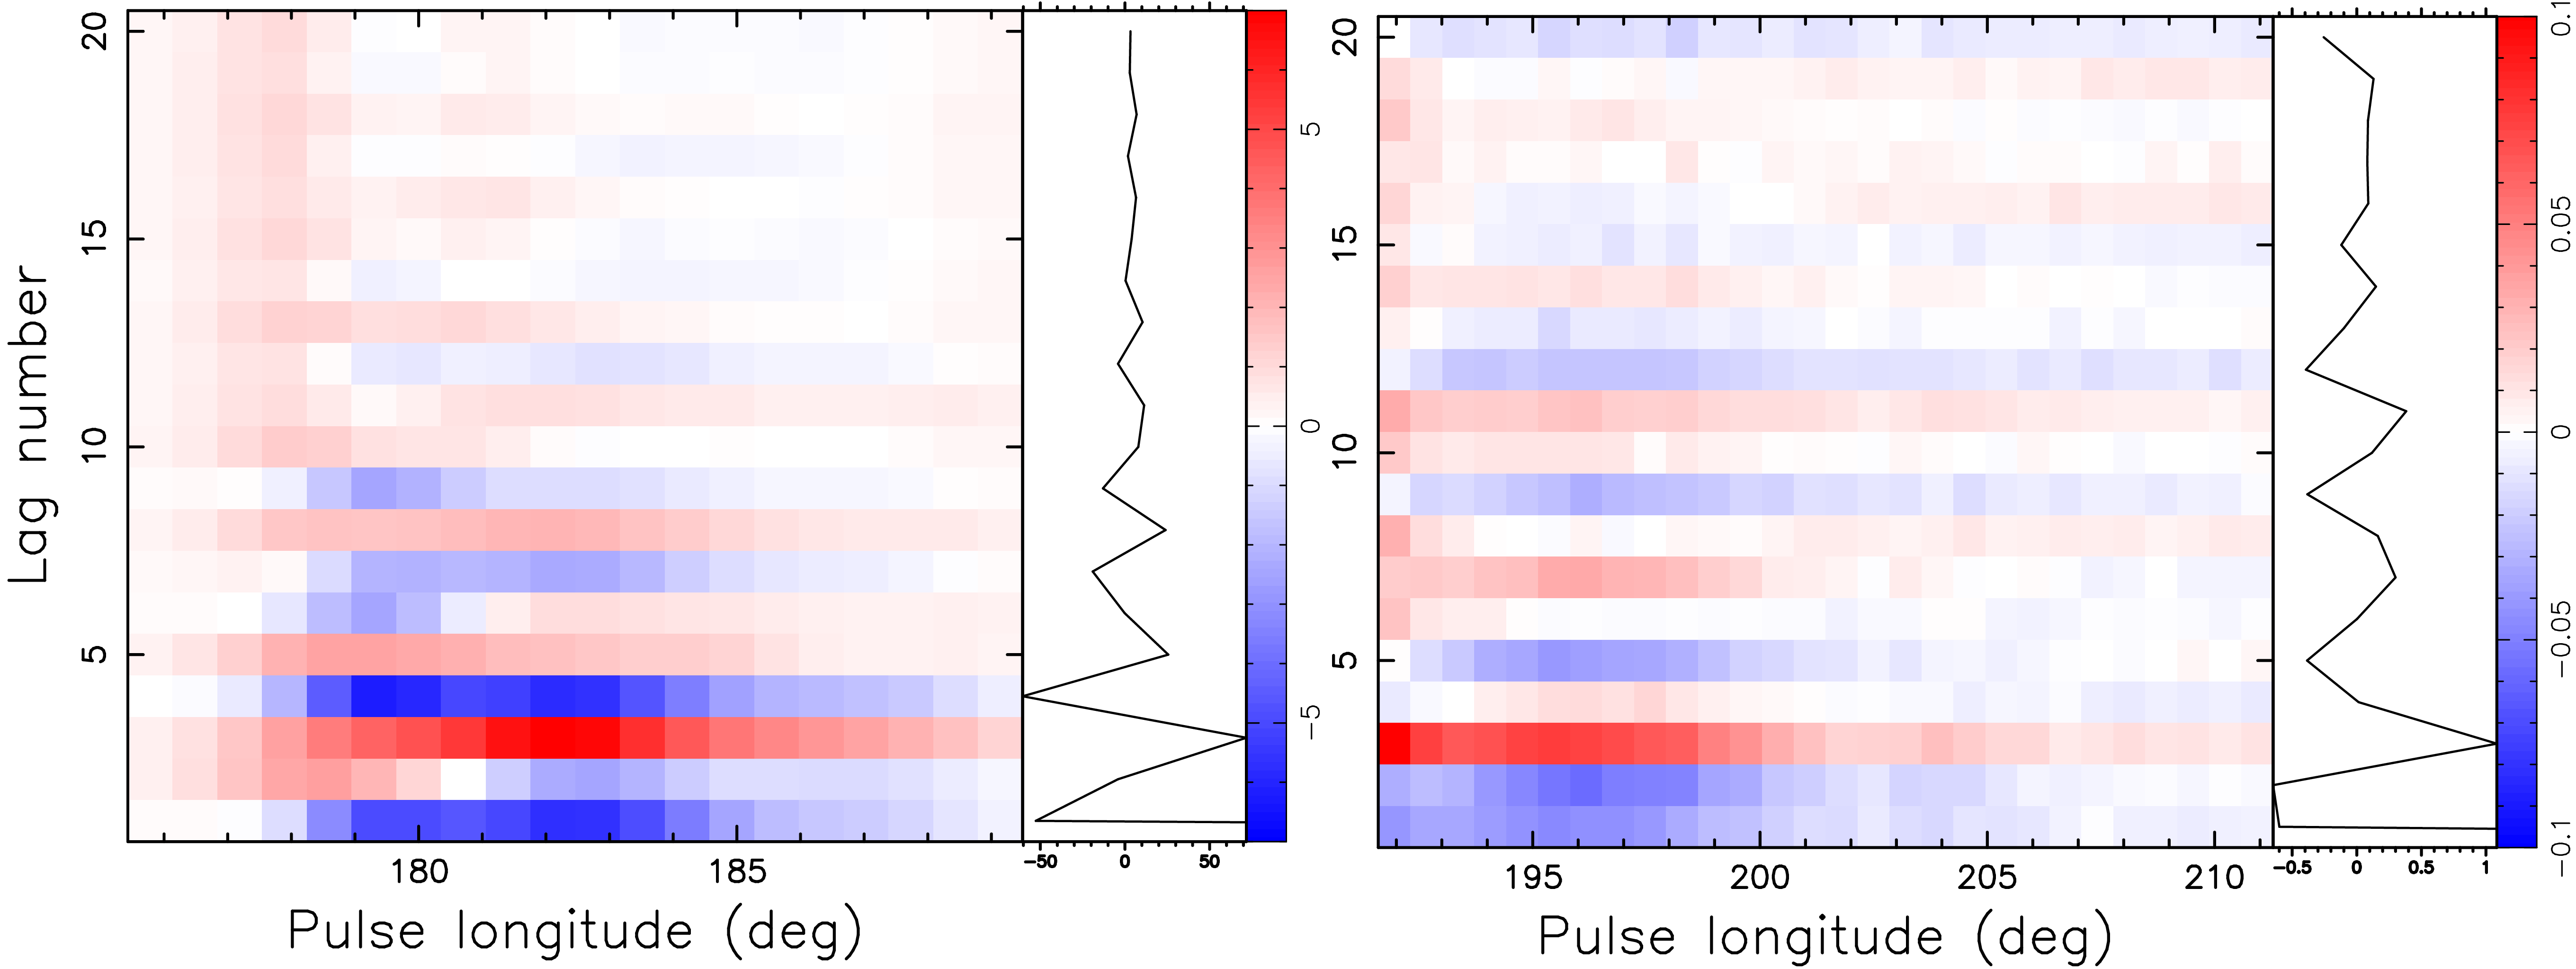
\includegraphics[width=\textwidth]{Figures/J1518/LRAC}
        \caption[The longitude-resolved autocorrelation spectrum]{The LRAC for lags 1--20, plotted between pulse longitudes $176\degr$ and $190\degr$ (left panel) and $192\degr$ and $212\degr$ (right panel). Positive values are shown in red, and negative values are blue. The side panels show the integrated spectrum across the window.}
        \label{fig: J1518 - LRAC}
    \end{center}
\end{figure}
The LRAC peaks at lag 3 for both longitude ranges, however the changing periodicity across the profile is evident. The gradual decrease in $P_3$ between profile components C1 and C2 is evident in the left-hand panel, revealed by the way the peak in the autocorrelation (with lag) changes. In the left-hand side panel the first maximum in the LRAC occurs between a lag of 2 and 3 pulses at the earlier longitudes, shifting to a lag of 3 pulses for most of the pulse longitude range. The minimum occurs at a lag of 4 pulses. In the second panel the first maximum again occurs at a lag of 3 pulses, with the following minimum at a lag of five pulses. This is consistent with the steady decrease in the modulation frequency observed with pulse longitude in the LRFS. In profile component C1 ($180\degr$), periodicities at both 0.07~cpp and 0.38~cpp are observed. Unfortunately the 0.07~cpp modulation is relatively weak, and its effect on the LRAC is too small to be recognised.

\begin{figure}
    \begin{center}
        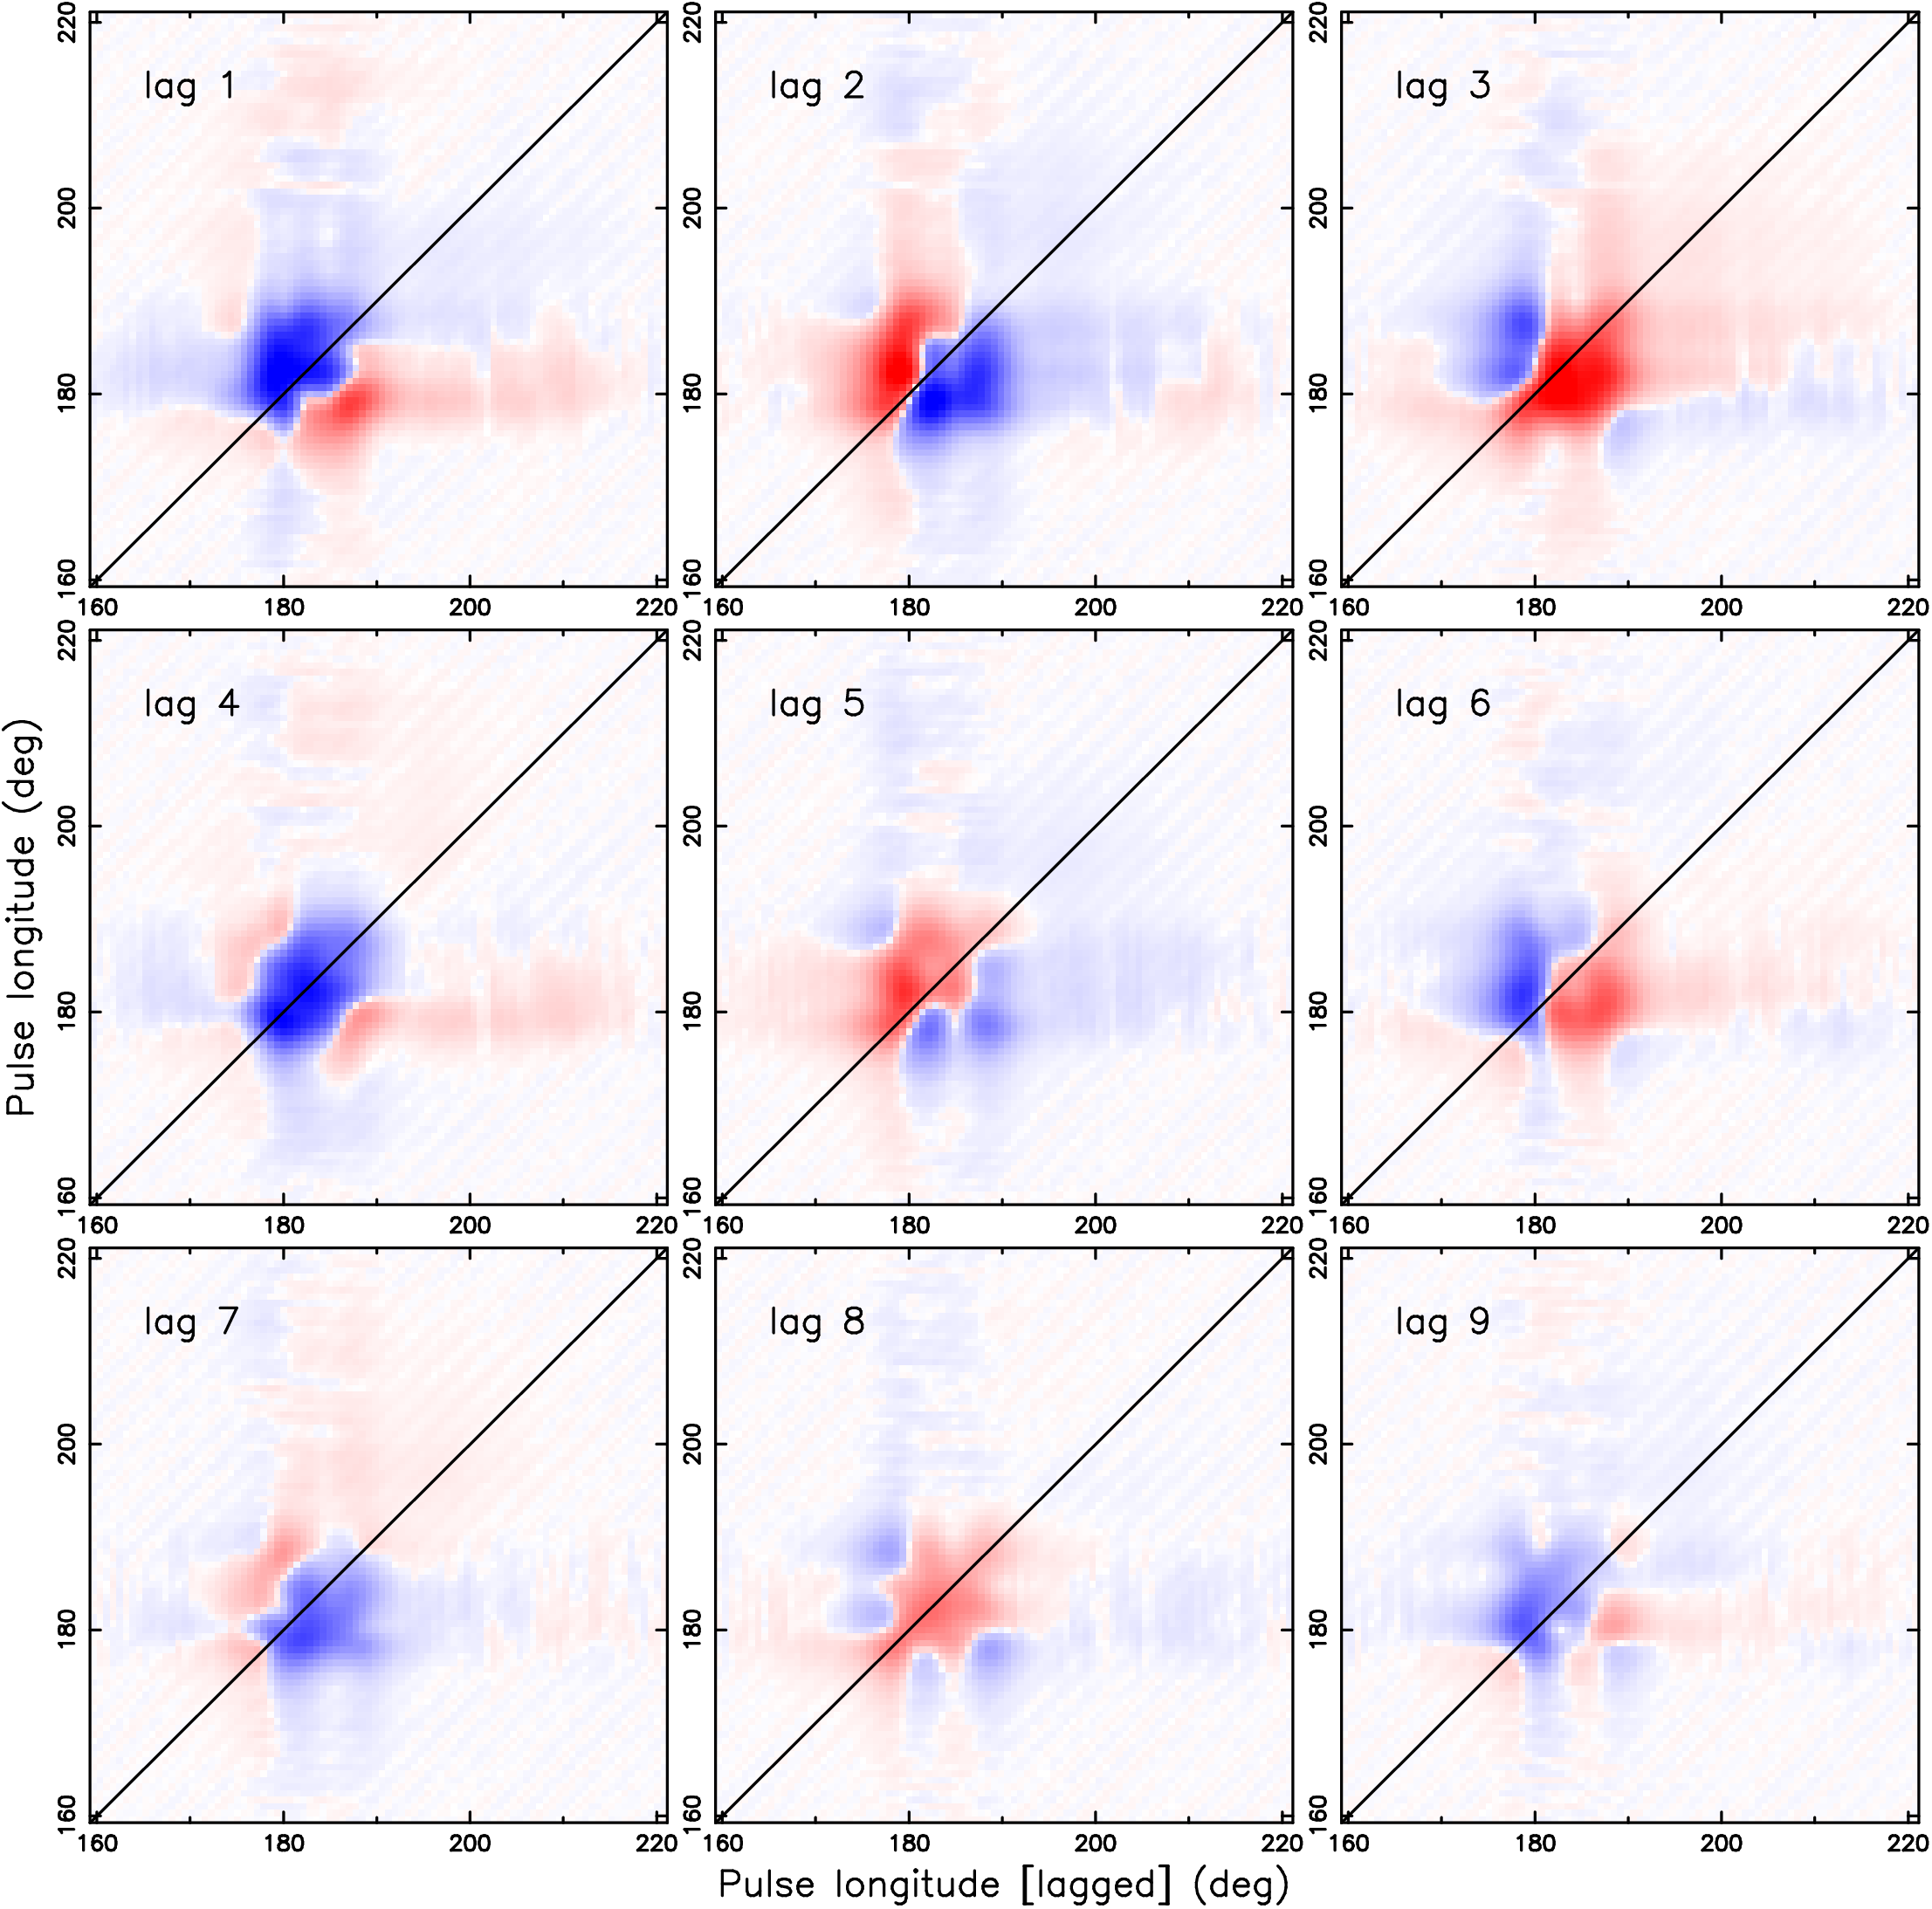
\includegraphics[width=1.0\textwidth]{Figures/J1518/LRCC}
        \caption[The longitude-resolved cross-correlation spectrum]{The LRCC is shown for lags 1--9 for the main profile between pulse longitudes $160\degr$ and $220\degr$. As with the LRAC, positive values are shown in red, and negative values are blue.  The diagonal black lines connect matching pulse longitude bins, so represent autocorrelations.}
        \label{fig: J1518 - LRCC}
    \end{center}
\end{figure}
The shift in modulation frequency with pulse longitude also manifests itself in the LRCC which is shown in Fig.~\ref{fig: J1518 - LRCC}, for lags ranging from 1 to 9. The diagonal black line in each panel connects bins with the same pulse longitude in the lagged and non-lagged pulse sequence, so represent the autocorrelation as seen in Fig.~\ref{fig: J1518 - LRAC}. As with the LRAC, the colour scale represents the correlation coefficients, with positive values denoted by red shading and negative values by blue. Correlations become anti-correlations and vice-versa as the lag number increases, corresponding to the rapid $0.38$~cpp modulation. The shifting position of the division between positive and negative correlations with pulse longitude implies drifting across the profile. As not all profile components fluctuate at the same frequency, this manifests itself as the emergence of more complex patterns in the later lags. These are fainter overall as the periodicities do not remain coherent over long timescales and so smear out any structure. Non-zero correlation coefficients are also faintly visible in a `$+$' structure in each panel, centred on the main profile components. It is unclear what the interpretation of this is, although it may be due to baseline variations on length scales slightly shorter than the pulse period (long-term variations were removed as described in Sec.~\ref{sec: J1518 - analysis - disjoint modes}).

There is some faint diagonal striping visible in the background of each panel which is the result of low-level, extremely rapid artificial baseline variations. These must be present throughout the observation as it is seen at all pulse longitudes. These are too weak to be a problem in any of the analysis presented in this work.




















\section{Discussion and conclusions}
\label{sec: J1518 - discussion}

\subsection{New profile components}
\label{sec: J1518 - discussion - new profile components}

The newly identified components in the integrated profile (C4 and C5, see Fig.~\ref{fig: J1518 - integrated profile}) greatly increase the fraction of the rotation period over which emission is detected (its `duty cycle'). The stronger of the two, C5 (at $\sim$275$\degr$), appears to be connected to the main component by a faint bridge of emission, which suggests that this is all part of the same emission region. If this is the case then the `main' profile width is extended to span at least $\sim$150$\degr$, or 0.42 pulse phase (estimated by measuring the region between components C1 and C5 where the pulsar emission is clearly visible over the background noise). The much weaker leading component C4 is consistent with being completely separate from the main profile, and could potentially be associated with emission from the opposite magnetic pole (i.e. an interpulse) as it is separated from the centre of the main profile by 165$\degr$, so roughly half a stellar rotation. If this is true, then that would suggest that PSR~J1518+4904 has a high magnetic inclination angle $\alpha$ that allows emission from both poles to be viewed. On the other hand, the main profile spanning C1--C3 and C5 is extremely wide, meaning that the emission beams themselves must be very wide (or the magnetic inclination angle $\alpha$ is extremely small). In the two-pole scenario, the narrow interpulse component C4 suggests the line-of-sight is only grazing the interpulse beam, meaning $\alpha$ may not be too large after all. Simultaneous observations of PSR~J1518+4904 covering a wide range of frequencies -- as performed for PSR~J0250+5854 in Chapter~\ref{chapt: J0250} -- would be very useful in exploring effects such as radius-to-frequency mapping that can be used to constrain the viewing geometry.

The new components do not appear to evolve much with frequency or time -- apart from the distinct change of the relative amplitude of component C2, which becomes brighter towards the top of the band relative to the other components (central panel of Fig.~\ref{fig: J1518 - profile frequency evolution}). This behaviour was seen by \citet{KLL+1999} in data taken with the 100~m Effelsberg telescope, and they noted that this component initially weakens between 370 and 610 MHz before increasing to become dominant at 1.8~GHz. In this work they also observe that the small, tertiary component of the main peak (around $210\degr$ pulse longitude in our figures) is stronger at low frequencies before fading out completely at 1.4~GHz. This is in contrast to their earlier observations using the same telescope \citep{KXL+1998} where this feature was discovered again at 1.4~GHz. The difference between these two data sets is that the later observations (between July 1997 and October 1998) were coherently dedispersed whereas the earlier observations (around April 1994) were not, although it is unclear why this should mean the tertiary profile component should disappear. Regardless, it is clearly present in the incoherently dedispersed FAST data, so this feature may vary in intensity over timescales of years. 










\subsection{Single-pulse modulation properties}
\label{sec: J1518 - discussion - funky P3}

The S2DFS (Fig.~\ref{fig: J1518 - S2DFS}) shows that the broadness of the modulation frequency peaks in the spectra is due to stochastic variation of the modulation frequency over unresolved timescales (i.e. smaller than 256 pulses). Stochastic variability is observed at all pulse longitudes.

The apparent change in $P_3$ as a function of pulse longitude is extremely unusual. The shift in $P_3$ with longitude is stable in time (Fig.~\ref{fig: J1518 - drifting P3 components}) and frequency (e.g. Fig.~\ref{fig: J1518 - lrfs freq evolution}). There is a trend where the 0.38~cpp component decreases slightly in fluctuation frequency and power between profile components C1 and C2 whilst the distribution of frequencies becomes broader. The 0.28~cpp periodicity that exists between C2 and C3 may be a continuation of this trend, although it seems to be a distinct feature. This more narrow feature is significantly offset from the main component at $P_3 = 2.659\pm0.008P_1$. We considered the idea that this is down to the presence of two distinct drift modes in PSR~J1518+4904, as seen for example in PSR~B0031$-$07 (Chapter~\ref{chapt: B0031}). The length of the FFT used in calculating the S2DFS (Fig.~\ref{fig: J1518 - S2DFS}) was 256 pulses, so if mode-switching were occurring on faster timescales it would not be resolved by this analysis.

It is also curious that the modulation feature at 0.28~cpp appears to be significantly weaker in the 2018-08-04 observation, without affecting the overall intensity, whilst the modulation features at 0.38~cpp and 0.07~cpp appear to be just as strong (see Fig.~\ref{fig: J1518 - lrfs time evolution}). It is highly unusual for pulsars to show time-dependent variation in modulation power (with the exception of mode changes). We hypothesised that this modulation feature could be present for only part of the observation, accounting for its overall weakness in the (time-averaged) LRFS; however, a S2DFS revealed that it is present throughout (but very weak). %\todo{Crispin non-thesis comment: I wonder if a this suggests that modulation is not caused by periodic brightening of the emission (such as the sparks of the carousel model) on a constant background, but rather both brightening and dimming about a mean value? Not sure how to test this.}

In the majority of pulsars, if periodic single-pulse fluctuations occur, they do so with the same periodicity across all profile components, although stochastic variation about the mean frequency is common. This has been demonstrated by \citet{Wxxx2007} who studied the LRFS and 2DFS for 187 pulsars. Some pulsars exhibit coherent drifting with very stable values of $P_3$, whereas the diffuse drifters more closely resemble what is seen for PSR~J1518+4904. There are a number of pulsars for which multiple distinct $P_3$ spectral features are seen, however these are attributed to mode changes, as many of them were previously known to do so. The 2DFS of PSR~B1929+10 at a wavelength of 21~cm was found to have two broad features with an opposite drift sense at different $P_3$ values, not unlike PSR~J1518+4904. These features were also observed by \citet{Bxxx1973} in the LRFS. A negative $P_2$ was detected for the short-period modulation feature, but the longer-period feature had a positive drift sense, and both were associated with the same profile components. The conclusion reached was that PSR~B1929+10 switches between drift modes with different $P_3$, and that the two modes have opposite drift directions. Seven pulsars were shown to have opposite drift directions in different components: PSRs B0450+55, B1540$-$06, B0525+21, B1839$-$04, B2020+28, B0329+54, and B1237+25. The $P_3$ values of these were the same however, and so their `bidrifting' may be attributed to non-circular carousels of sub-beams \citep[e.g.][]{QLZ+2004, Wxxx2016, WWxx2017, SLWM2020}.

Mode-changing behaviour is primarily associated with normal, non-recycled pulsars, with periods greater than 100 milliseconds. Nevertheless, total intensity and polarisation profile morphology changes have been observed in four recycled pulsars: PSRs J1022+1001, J1730$-$2304, B1821$-$24, and J2145$-$0750 \citep{KXC+1999}. The cause of the changes was determined to be intrinsic to the pulsars rather than due to propagation or hardware effects, and the authors stress that they are \textit{not} consistent with the mode-changing behaviour of normal pulsars -- for PSR J1022+1001, the profile changes occurred smoothly over hundreds of thousands of pulses. In normal pulsars, even those that exhibit mode changes, integration over $\sim$10,000 pulses are typically sufficient to produce a stable profile \citep{HMTx1975, RRxx1995}. Two of the four (PSRs J1022+1001 and J2145$-$0750) have an orbiting companion whereas the other two do not, implying that their profile changes are not necessarily due to them being in a binary system. Overall, the cause of the phenomenon could not be determined. 

Mode changing was robustly identified by \citet{MKMP2018} in PSR~B1957+20, a MSP with a period $P_1=1.6$~ms. This pulsar switches between two distinct modes on an average timescale of 1.7 seconds, the shortest mode-switching time observed to date. In units of pulse periods this timescale of $\sim 1000 P_1$ is not dissimilar to mode switching in normal pulsars though. PSR~B1957+20 has a narrow, single-component main pulse and a broad interpulse with two components. The main pulse is largely unaffected by the mode change, but the interpulse decreases in intensity, and its two components change in relative intensity. This change in relative intensity was the signature of mode switching we searched for in PSR~J1518+4904 by analysing the correlated changes in the flux density of the two regions of the profile that have different $P_3$ values in the LRFS (Fig.~\ref{fig: J1518 - energy scatter plots}). No bimodality could be seen in the distribution of either component separately, nor when combined in a scatter plot of both quantities.

As discussed extensively in Chapt.~\ref{chapt: B0031}, the carousel model is the most well-known and developed model of for sub-pulse drift. It can explain many of the commonly observed features of subpulse drifting, by modelling the subpulses as a pattern of sub-beams that circulates around the magnetic axis \citep[e.g.][]{RSxx1975, DRxx1999, GSxx2000, GMGx2003}. The circulation of the carousel is the result of an $\mathbf{E} \times \mathbf{B}$ drift \citep{RSxx1975}. If drifting occurs at varying altitudes in the magnetosphere where the fields are different, this could potentially explain slight shifts in $P_3$ over time. However, this is distinctly different from the standard picture where the drift arises because of $\mathbf{E} \times \mathbf{B}$ in the polar gap near the surface, which causes the sites (`sparks') of particle injection into the magnetosphere to drift, resulting in a corresponding drift of the radio emission generated at higher altitudes. %\todo{MELROSE PAPER ABOUT MAGNETOSPHERE-WIDE DRIFT - DIFFERENTIAL ROTATION?}

Even without invoking differences in the circulation period of the carousel $P_4$, discrete changes in $P_3$ could arise if the number of sub-beams can change. The alias effect which occurs for fast circulation (see for example Appendix~\ref{app: geometry derivations}) can explain subsequent reversals in the drift direction \citep[e.g.][]{Wxxx2007}. Simultaneous drifting at two different $P_3$ values in different profile components could hypothetically occur when nested carousels are considered, as is the case in the core-cone model \citep[e.g.][]{Rxxx1983a, Kxxx1994, GGxx2003}. If the nested carousels either circulate with different periods or have a different number of sub-beams, different $P_3$ values are predicted to be observed simultaneously. However, the question is why this should be the case for PSR~J1518+4904 and not frequently observed in the broader population? Furthermore, in such a model we might expect some degree of symmetry about the fiducial plane (see Chapter~\ref{chapt: B0031}) in terms of the emission properties (a symmetric pattern of $P_3$ values as a function of pulse longitude is implied for example). Such symmetry is entirely absent in PSR~J1518+4904. 

An alternative mode for single-pulse modulation is non-radial oscillations of neutron stars. Originally proposed as the source of radio emission in pulsars \citep{Rxxx1968}, these were later suggested as the possible origin of drifting subpulses \citep{DCxx1968}, revised by \citet{CRxx2004}. Although they provide a natural explanation for phenomena such as discontinuities in subpulse phase (similar to the feature observed in PSR~J1926$-$0652; Chapter~\ref{chapt: J1926}), nulling, and mode changing, fine tuning is required to explain the longitude-dependence of $P_2$ commonly seen in driftbands.  Although a drift direction reversal can in principle be explained as a change in the beat frequency between oscillation and stellar rotation, the model struggles to explain pulsars that exhibit modulation with opposite drift directions in different components simultaneously.

Whilst discrete changes in $P_3$ as a function of longitude can hypothetically be attributed to unresolved mode changes (although we have found no evidence for any), the apparent smooth change between profile components C1 and C2 (Fig.~\ref{fig: J1518 - drifting P3 components}) cannot be explained. It cannot occur under the carousel model as it would require a smooth variation of circulation rate at different locations. If differential rotation is possible in pulsar magnetospheres it is unclear how any sub-beam-like structure can be maintained as a function of magnetic azimuth. Any distinct pattern would rapidly be smeared out, so a mechanism should exist to regenerate the pattern in order for circulation to be observable as drifting subpulses. If that is the case, it is unclear why the same number of beamlets are being regenerated each time, and hence why the same periodicities are being observed over extended periods.


In conclusion, we have discovered curious modulation properties for PSR~J1518+4904. In particular, the longitude-dependent modulation observed in part of the profile is unique in the pulsar population. This finding presents some serious challenges for existing models of pulsar emission and how they can explain the observed pulse-to-pulse variability in radio pulsars. The work in this chapter has shown that this pulsar merits further observations with FAST, which is currently fully commissioned and operational with good polarisation capabilities (see Chapter~\ref{chapt: J0250}), and a proposal to do so has been submitted. These observations could establish with certainty whether the observed modulation effects are indeed fully associated with changes in Stokes $I$, or if some of the variability arises because of periodic changes in polarisation. This could add an additional layer of complexity to an already problematic-to-interpret dataset.


